\section{Développement du firmware} \label{sec:Dev-firmware}

Lors de cette section, nous décrirons le processus de développement du firmware du PIC32. Les décisions prises seront expliquées et les différents algorithmes seront illustrés et décrits.

En premier lieux nous allons analyser lors de la section \ref{ssec:ProtocolGNSS} comment traiter les données du \gls{gnss}, il s'agit d'un élément critique.


\subsection{Protocoles du GNSS} \label{ssec:ProtocolGNSS}
Il existe différents protocoles pour le format de données de localisation. Le \textbf{CAM-M8C-0} supporte plusieurs protocoles, visibles sur la figure \ref{fig:protocolsGNSS} :

\begin{figure}[h]
	\centering
	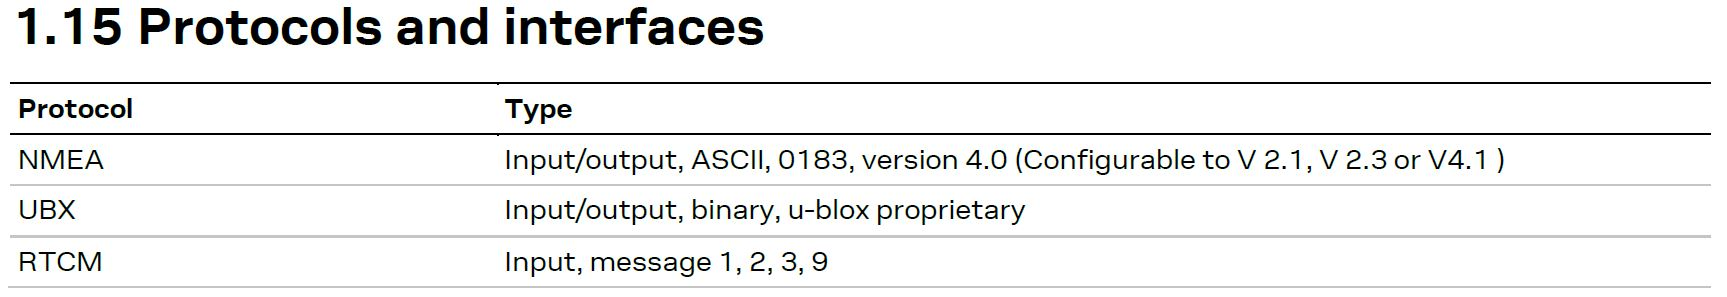
\includegraphics[width=.75\linewidth]{../figures/code/Protocols}
	\caption{Protocoles disponibles.}
	\source{\Gls{datasheet} du \href{https://content.u-blox.com/sites/default/files/CAM-M8-FW3\_DataSheet\_\%28UBX-15031574\%29.pdf}{CAM-M8C-0}}
	\label{fig:protocolsGNSS}
\end{figure} \vspace{-4mm}

\begin{tabularx}{\textwidth}{llX}
	\textbf{NMEA}& : & Norme établie par la \textit{National Marine Electronics Association}. Elle suit un format \fbox{\textbf{ASCII}}. \\
	\textbf{UBX} & : & Format propriétaire de u-blox avec des données \fbox{\textbf{binaires}}. Il permet d'envoyer des trames de configuration. \\
	\textbf{RTCM} & : & Protocole pour des données GPS différentielles. Établi par la \textit{Radio Technical Commission for Maritime Service}.
\end{tabularx} 


Le \textbf{CAM-M8C-0} est configuré, par défaut, pour envoyer des messages au format NMEA, comme illustré sur la figure \ref{fig:default-messages}. \vspace{+2mm}

\begin{figure}[!h]
	\centering
	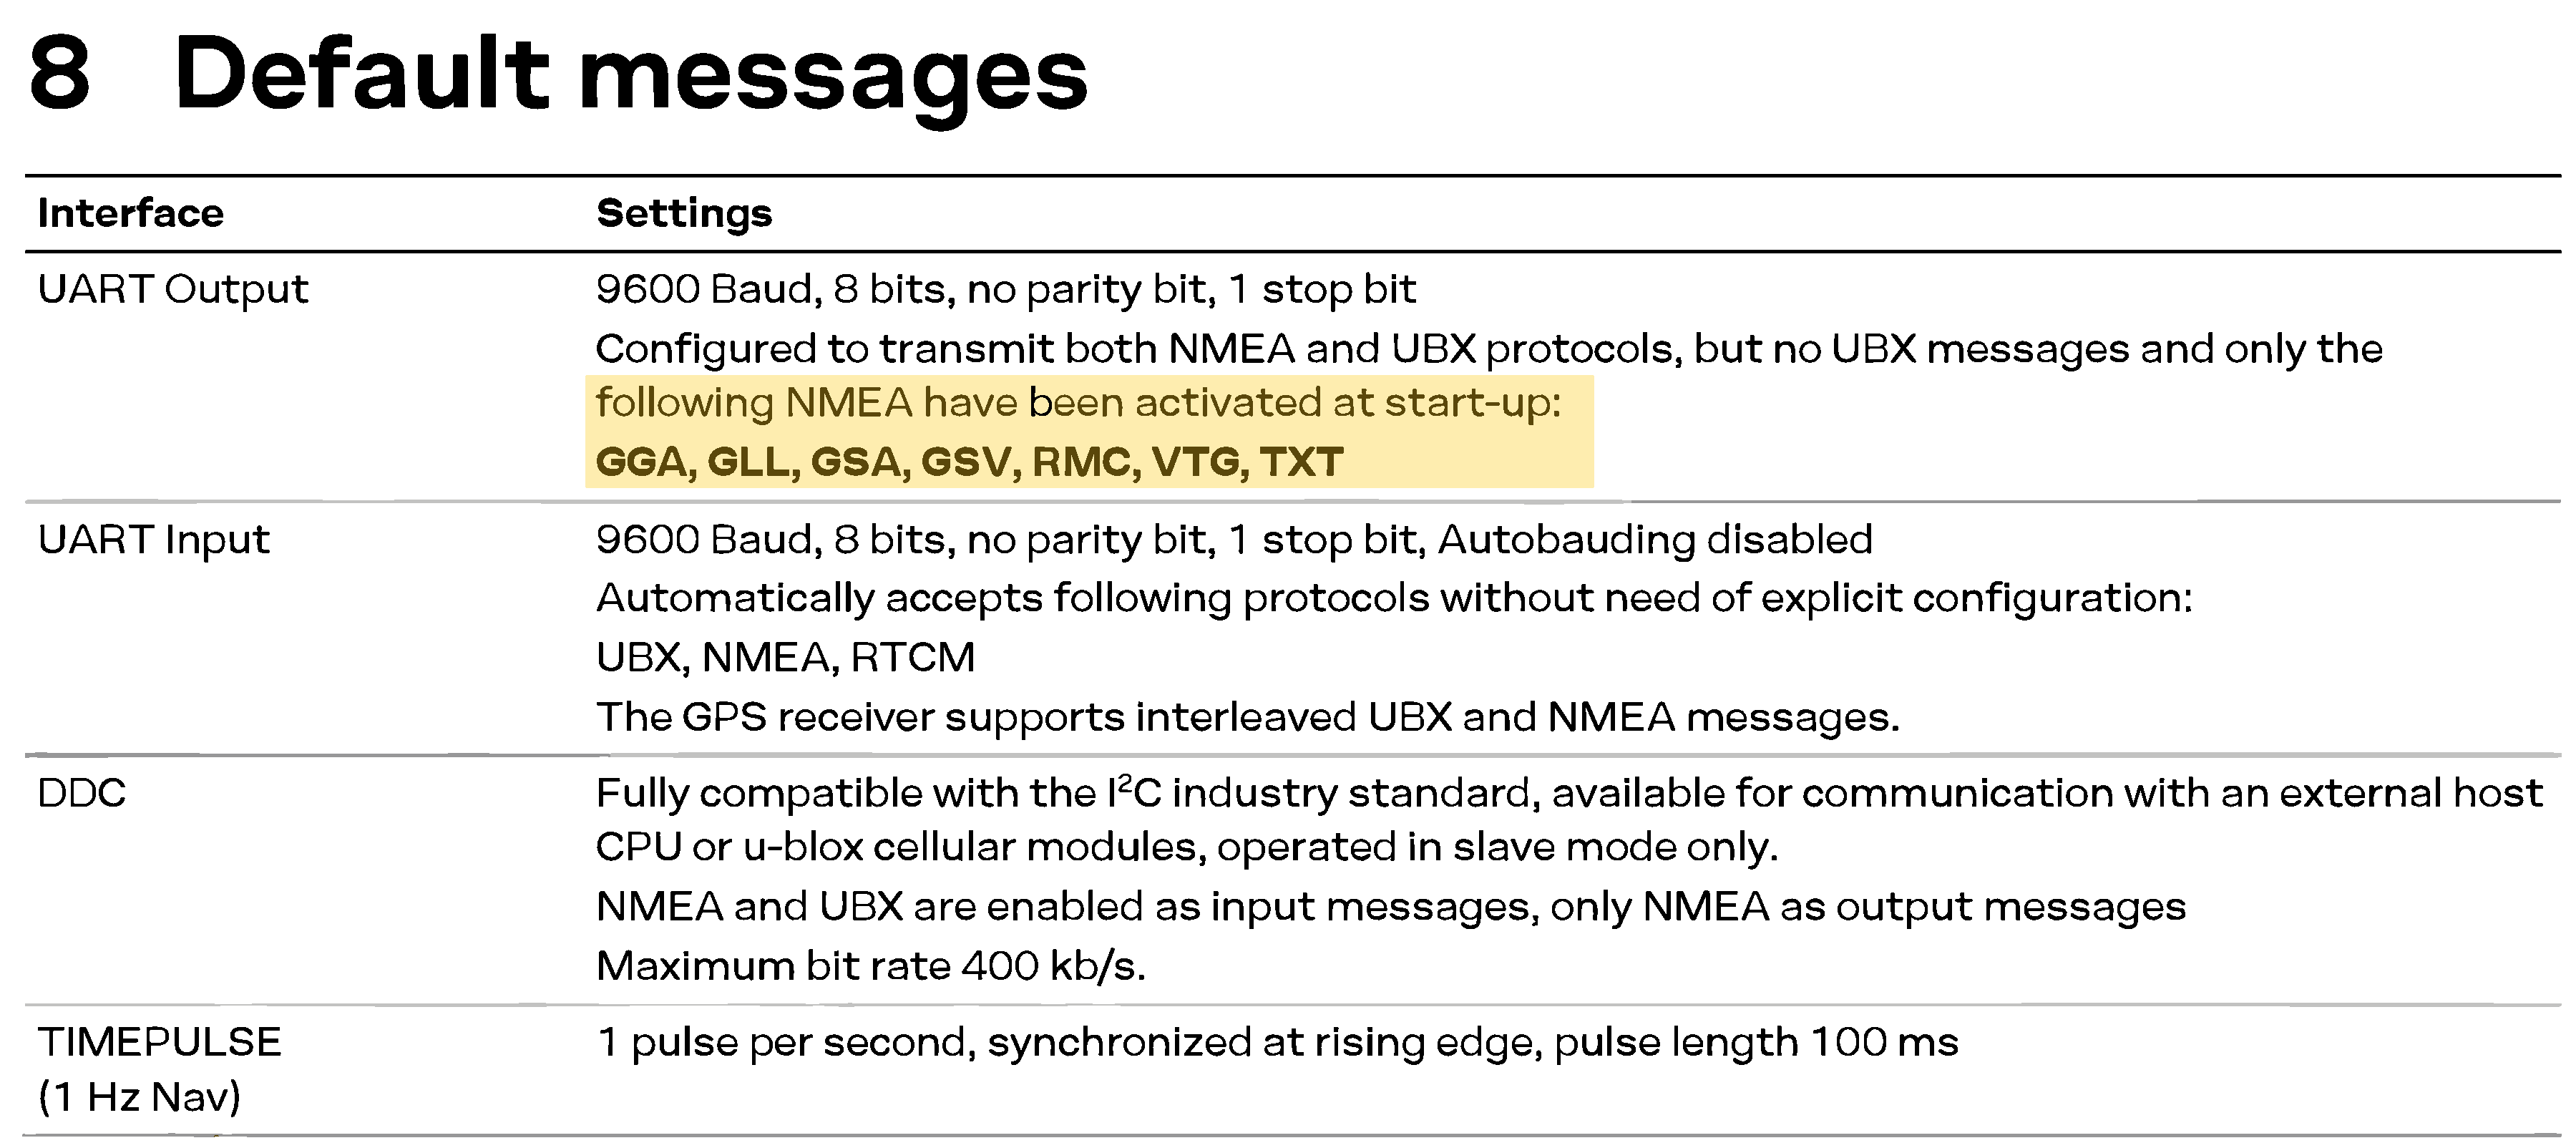
\includegraphics[width=0.7\linewidth]{../figures/code/Default-messages}
	\caption{Protocole par défaut.}
	\source{\Gls{datasheet} du \href{https://content.u-blox.com/sites/default/files/CAM-M8-FW3\_DataSheet\_\%28UBX-15031574\%29.pdf}{CAM-M8C-0}}
	\label{fig:default-messages}
\end{figure}

\clearpage

\subsubsection{Messages NMEA}
Comme nous avons pu constater sur la figure \ref{fig:default-messages}, il y a plusieurs messages \textbf{NMEA} : 

\textbf{GGA, GLL, GSA, GSV, RMC, VTG, TXT}

Ceux-ci sont décris dans le \href{https://www.ekf.de/c/cgps/cg2/inf/nmea_reference_manual.pdf}{manuel de référence du protocole NMEA} sur la figure \ref{fig:messages-nmea}

\begin{figure}[h]
	\centering
	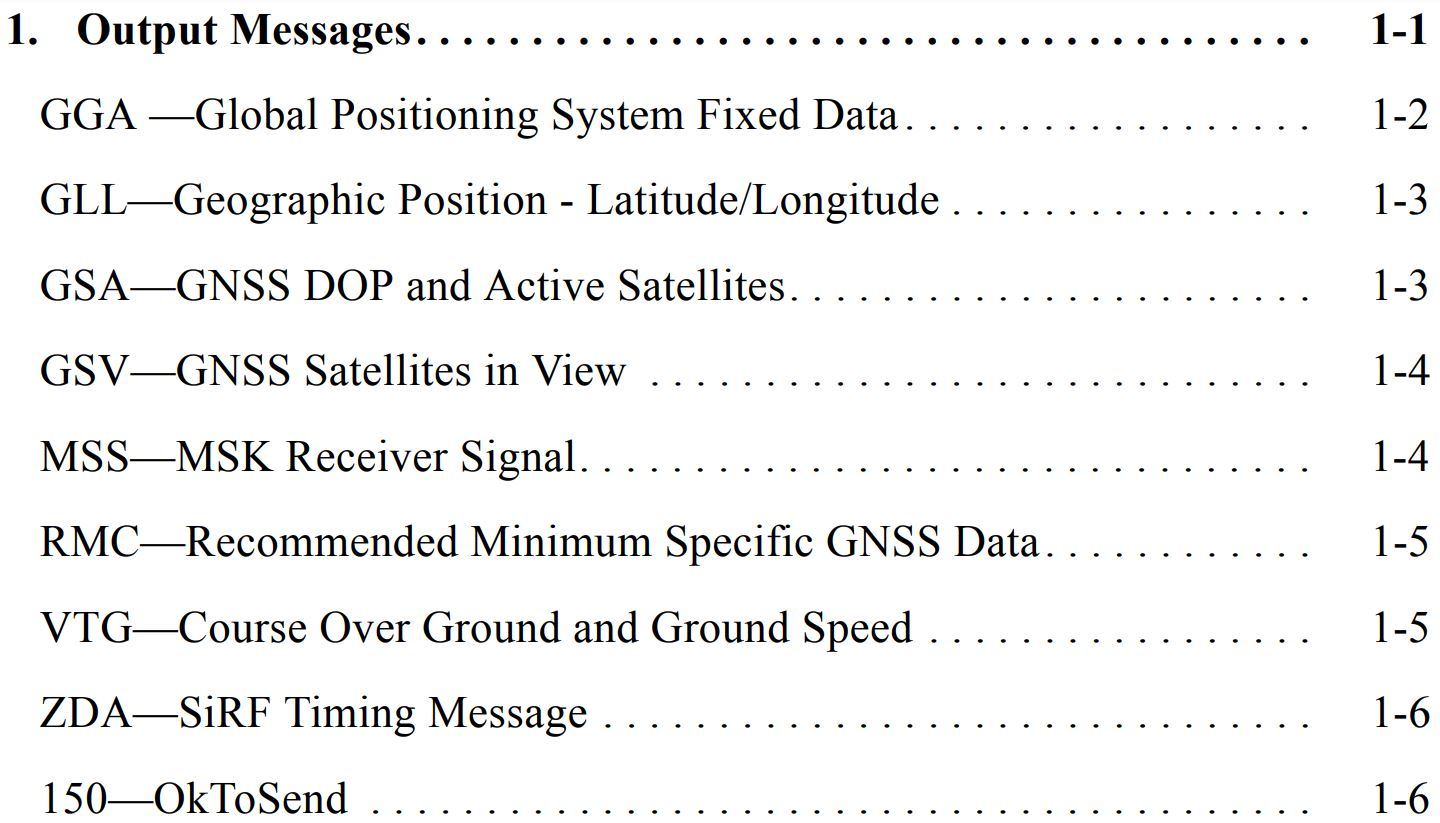
\includegraphics[width=0.55\linewidth]{../figures/code/Messages-NMEA}
	\caption{Messages NMEA.}
	\source{\href{https://www.ekf.de/c/cgps/cg2/inf/nmea_reference_manual.pdf}{Manuel du protocole NMEA}}
	\label{fig:messages-nmea}
\end{figure}

Les différents messages de la figure \ref{fig:messages-nmea} présentent des différentes données sous divers formats. Les messages peuvent être activés ou désactivés en configurant le module u-blox.

\subsubsection{Interprétation des données NMEA}
Avant d'avoir le \gls{pcb} monté et exploitable, sachant que nous connaissons le protocole par défaut du module, nous pouvons analyser des données \textbf{NMEA} pour mieux les comprendre et les traiter par la suite. Pour ce faire, le site \href{https://www.nmeagen.org/}{https://www.nmeagen.org/} permet de générer des coordonnées avec le protocole \textbf{NMEA}.

\begin{figure}[h]
	\centering
	\includegraphics[width=.75\textwidth]{../figures/code/map-localisation}
	\caption{Application d'une localisation NMEA.}
	\source{\href{https://www.nmeagen.org/}{nmeagen.org}, aéroport de La Blécherette, Lausanne}
	\label{fig:map-localisation}
\end{figure}

Sur la figure \ref{fig:parsed-nmea}, les messages de la figure \ref{fig:map-localisation} sont décodés via un \href{https://swairlearn.bluecover.pt/nmea_analyser}{analyseur NMEA en ligne}.

\begin{figure}[h]
	\centering
	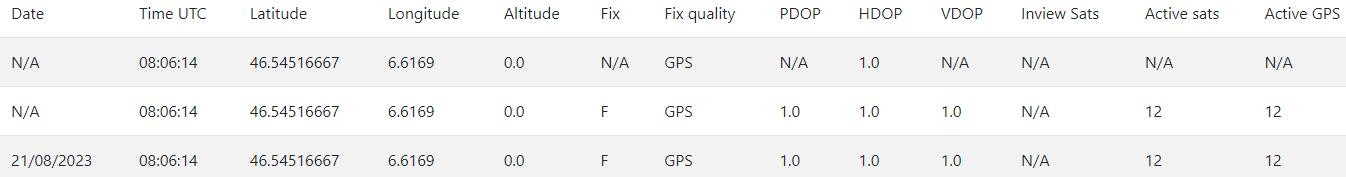
\includegraphics[width=0.8\linewidth]{../figures/code/parsed-nmea}
	\caption{Messages NMEA décodés.}
	\source{\href{https://swairlearn.bluecover.pt/nmea_analyser}{NMEA online analyser}}
	\label{fig:parsed-nmea}
\end{figure}

\clearpage

\subsubsection{Code décodeur de trame NMEA}
Afin de développer le code du décodeur \textbf{NMEA}, la librairie \href{https://github.com/kosma/minmea}{\textbf{minmea}} de licence libre, a pu être utilisée, modifiée et adaptée. Un algorithme a ensuite été mis en place :

\begin{itemize}
	\item[\oldstylenums{1}] Lecture du type de message (\textbf{GBS, GGA, GLL, GSA, GST, GSV, RMC, VTG, ZDA});
	\item[\oldstylenums{2}] Parsing des valeurs correspondantes à l'ID du message;
	\item[\oldstylenums{3}] Sauvegarde des valeurs dans une structure.
\end{itemize}


\begin{code}
\caption{gnss\_posGet\_nmea(...), décodage \textbf{NMEA}.}
\label{code:posget-nmea}
\begin{minted}[breaklines]{c}
// Get message ID, strict
*msg_id = minmea_sentence_id(message, true);
// Parse message depending on ID
if (*msg_id == MINMEA_SENTENCE_GBS)
	minmea_parse_gbs(&sentences->gbs, message);
else if (*msg_id == MINMEA_SENTENCE_GGA)
	minmea_parse_gga(&sentences->gga, message);
else if ...
\end{minted}
\end{code}

Dans le code \ref{code:posget-nmea}, on fait appel à une fonction qui va masquer les caractères du type du message. Ensuite, selon le message dont il s'agit, on le décode de différentes façons.

\begin{code}
\caption{minmea\_parse\_gbs(...), décodage message \textbf{GBS}.}
\label{code:parse-gbs}
\begin{minted}[breaklines]{c}
bool minmea_parse_gbs(struct minmea_sentence_gbs *frame, const char *sentence)
{
	// $GNGBS,170556.00,3.0,2.9,8.3,,,,*5C
	char type[6];
	if (!minmea_scan(sentence, "tTfffifff",
			type,
			&frame->time,
			&frame->err_latitude,
			&frame->err_longitude,
			&frame->err_altitude,
			&frame->svid,
			&frame->prob,
			&frame->bias,
			&frame->stddev
			))
		return false;
	if (strcmp(type+2, "GBS"))
		return false;
	return true;
}

\end{minted}
\end{code}

Dans le code \ref{code:parse-gbs}, on masque les éléments du message selon son format, d'une manière similaire à la fonction standard \textit{\textbf{scanf(...)}}.

\clearpage

Les données spécifique au message \textbf{GBS} sont ensuite stockées dans une structure, que l'on peut observer dans le code \ref{code:struct-gbs}.

\begin{code}
\caption{Structure \textbf{GBS}.}
\label{code:struct-gbs}
\begin{minted}[breaklines]{c}
struct minmea_sentence_gbs {
	struct minmea_time time;
	struct minmea_float err_latitude;
	struct minmea_float err_longitude;
	struct minmea_float err_altitude;
	int svid;
	struct minmea_float prob;
	struct minmea_float bias;
	struct minmea_float stddev;
};
\end{minted}
\end{code}

Sachant que plusieurs types de messages peuvent être interceptés, chacune des structures des différents formats de messages est elle-même stockée dans une structure que l'on peut observer dans le code \ref{code:struct-msgs}.

\begin{code}
\caption{Structures messages.}
\label{code:struct-msgs}
\begin{minted}[breaklines]{c}
typedef struct minmea_messages{
	struct minmea_sentence_gbs gbs;
	struct minmea_sentence_rmc rmc;
	struct minmea_sentence_gga gga;
	struct minmea_sentence_gll gll;
	struct minmea_sentence_gst gst;
	struct minmea_sentence_gsa gsa;
	struct minmea_sentence_gsv gsv;
	struct minmea_sentence_vtg vtg;
	struct minmea_sentence_zda zda;
}minmea_messages;
\end{minted}
\end{code}

Les données sont ensuite traitées dans l'application. Pour paramétrer le \textbf{CAM-M8C-0}, des messages \textbf{UBX} peuvent être envoyés. Pour ce faire, des éléments de la librairie \href{https://github.com/u-blox/ubxlib}{\textit{ubxlib}} peuvent être repris, notamment les fonctions d'encodage et de décodage des messages \textbf{UBX}.



\subsection{Configuration des périphériques}
Les périphériques utilisés par le microcontrôleur doivent êtres paramétrés et initialisés. Le configurateur \gls{harmony} permet de le faire simplement.

\begin{figure}[h]
	\centering
	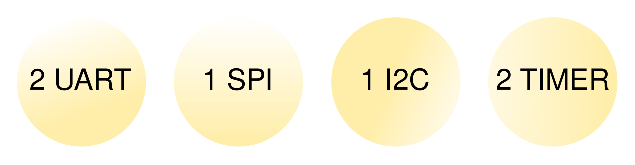
\includegraphics[width=.5\linewidth]{../figures/code/périphériques}
\end{figure}

\clearpage

\subsubsection{Timers}
Lors de cette section, 2 timers vont être configurés, ceux-ci ont des utilités différentes :

\begin{table}[h]
\begin{tabular}{lll}
	\textbf{Timer 1} & sert pour les attentes bloquantes précises. & 1 [$ms$] \\
	\textbf{Timer 2} & gère les délais entre les mesures et l'affichage des LEDs. & 10 [$ms$] \\
\end{tabular} 
\end{table} \vspace*{-5pt}

\underline{Dimensionnement timer 1}

$f_{sys} = 72\;MHz$

$f_{per} = 1\;kHz$

$presc = 8\;[-]$ \vspace*{-5pt}

\begin{equation*}
	C_{T1} = \frac{f_{sys}}{f_{per}*presc} - 1 = \frac{72*10^{6}}{1*10^{3}*8} - 1 = 8'999\; [-]
\end{equation*}


\underline{Dimensionnement timer 2}

$f_{sys} = 72\;MHz$

$f_{per} = 100\;Hz$

$presc = 16\;[-]$ \vspace*{-5pt}

\begin{equation}
	C_{T1} = \frac{f_{sys}}{f_{per}*presc} - 1 = \frac{72*10^{6}}{100*16} - 1 = 44'999\; [-]
\end{equation}

\begin{figure}[h]
	\centering
	\fbox{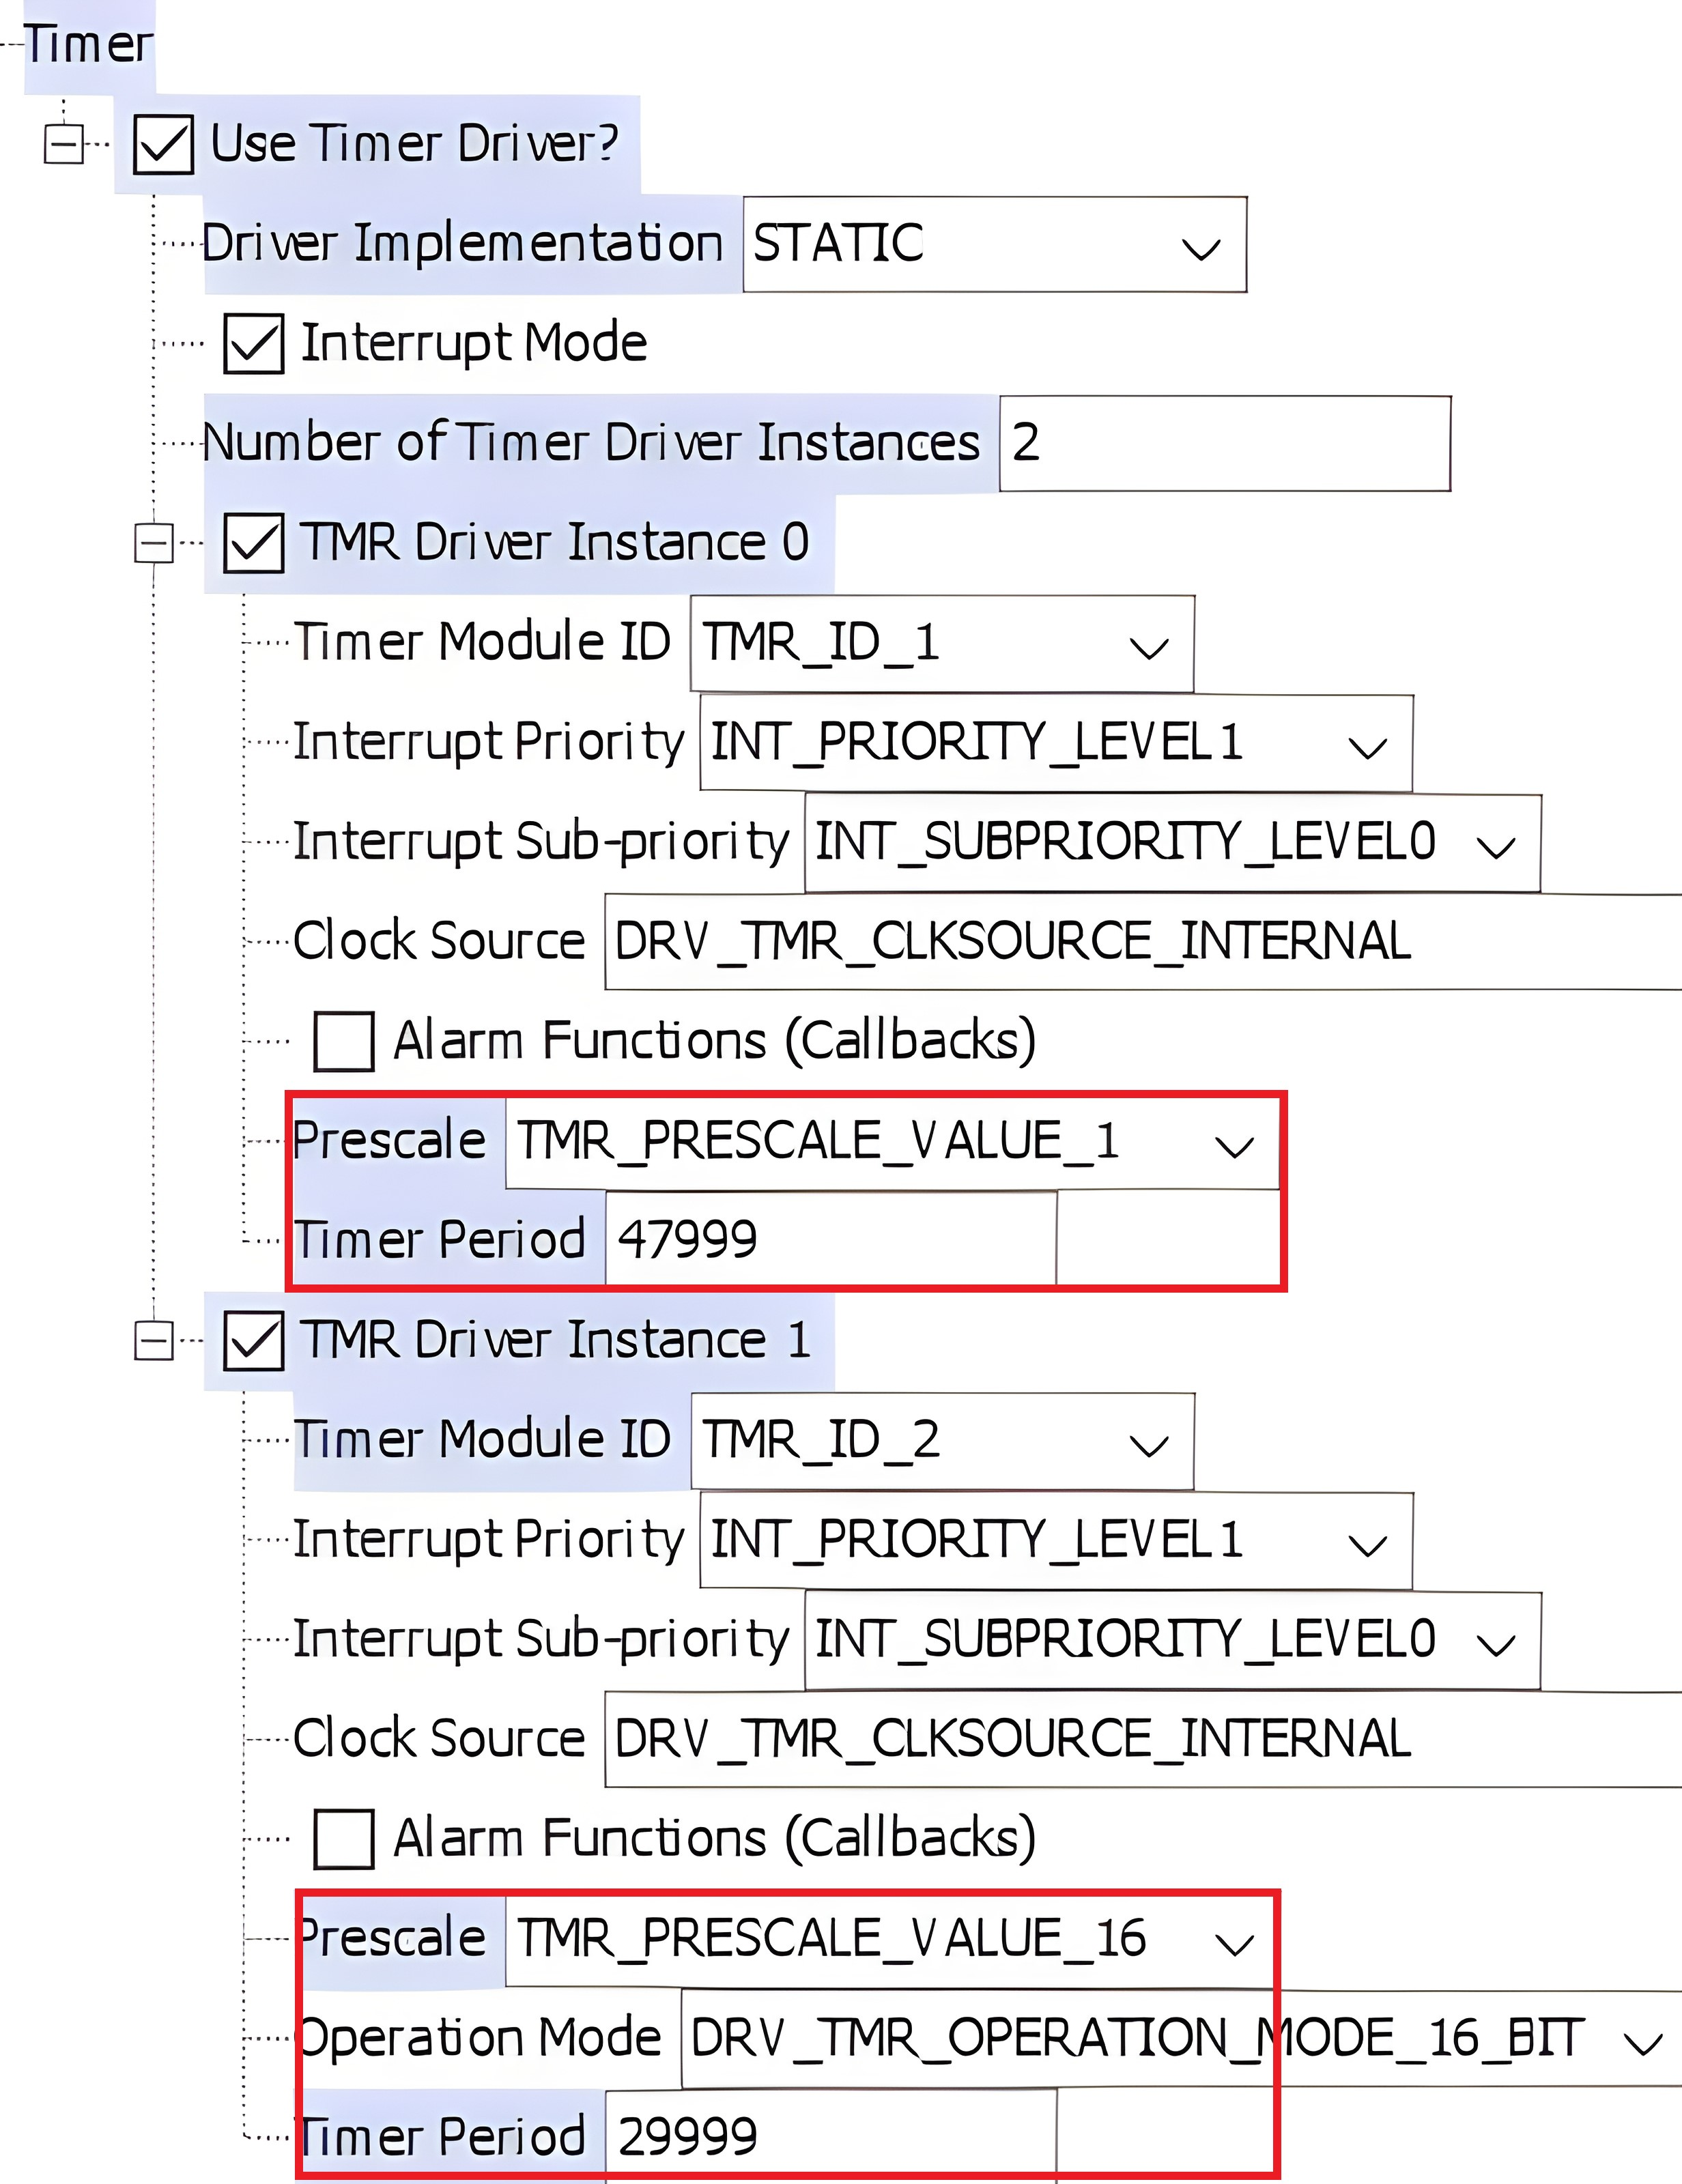
\includegraphics[width=.5\linewidth]{../figures/code/harmony/timers}}
	\caption{Configuration des timers.}
	\source{Auteur}
	\label{fig:timers}
\end{figure}

\clearpage

\begin{code}
\caption{Interruption \textbf{timer 1}, 1 [$ms$]}
\label{code:int-t1}
\begin{minted}[breaklines]{c}
void delayTimer_callback(){
	/* Increment delay timer */
	timeData.delayCnt ++;
}
\end{minted}
\end{code}

\begin{code}
\caption{Interruption \textbf{timer 2}, 10 [$ms$]}
\label{code:int-t2}
\begin{minted}[breaklines]{c}
void stateTimer_callback()
{
	/* Increment all counters */
	timeData.ledCnt ++;
	timeData.measCnt[BNO055_idx] ++;
	timeData.measCnt[GNSS_idx] ++;
	timeData.tmrTickFlag = true;
	/* When the button is pressed, the hold time is counted. */
	if(timeData.flagCntBtnPressed){
		timeData.cntBtnPressed++;
	}
	/* Do debounce on button every 10 ms */
	DoDebounce(&switchDescr, ButtonMFStateGet());
	/* Start a measure set each IMU period */        
	if ( ( timeData.measCnt[BNO055_idx] % (timeData.measPeriod[BNO055_idx]/10) ) == 0)
	timeData.measTodo[BNO055_idx] = true;
	
	/* Start a measure set each GNSS period */        
	if ( ( timeData.measCnt[GNSS_idx] % (timeData.measPeriod[GNSS_idx]/10) ) == 0)
	timeData.measTodo[GNSS_idx] = true;
	/* Manage LED if enabled */
	if((timeData.ledCnt >= LED_PERIOD) && (appData.ledState == true))
	LED_BOff();
} 
\end{minted}
\end{code}	

Dans le code \ref{code:int-t2}, nous pouvons voir le code de la routine d'interruption du timer 2. Lors de cette interruption, les différents compteurs de mesures sont incrémentés et différentes conditions vont tester si la période de mesure est atteinte. Une gestion du bouton a également lieu, notamment une mesure du temps d'appui, et une limitation des effets de rebonds mécaniques sur les signaux électriques observés par le \gls{mcu} par un échantillonnage diminué. Enfin, la LED de vie est gérée, notamment son temps allumé.

\clearpage

\subsubsection{USARTs}

Deux bus de communication UART ont dû être configurés dans le cadre de ce projet ; ceux-ci ont des utilités différentes.

\begin{center}
	\underline{Configuration des UARTs}
	\begin{table}[h]
		\centering
		\begin{tabular}{llllll}
			ID du BUS & Utilité & Baudrate & Interruption & Trame & Parité \\ 
			\hline
			UART ID1 & Réceptions commandes USB & 9600 & Priorité 1 & 8bits + 1stop & Non \\
			UART ID2 & Communication avec le \gls{gnss} & 9600 & Non & 8bits + 1stop & Non \\
		\end{tabular}
		\caption{}
		\label{tab:Usarts}
	\end{table}
\end{center}

L'USART ID1, mentionné dans le tableau \ref{tab:Usarts}, est configuré avec une interruption. Celle-ci a été mise en place afin d'implémenter un mécanisme de FIFO associé à un tampon de réception. Ceci facilite le traitement des données et évite leur perte lors de réceptions consécutives.

\subsubsection{Carte SD}
Harmony permet de configurer directement un périphérique carte-SD avec le bus SPI.
\begin{figure}[!h]
	\centering
	\begin{subfigure}[b]{0.5\textwidth}
		\centering
		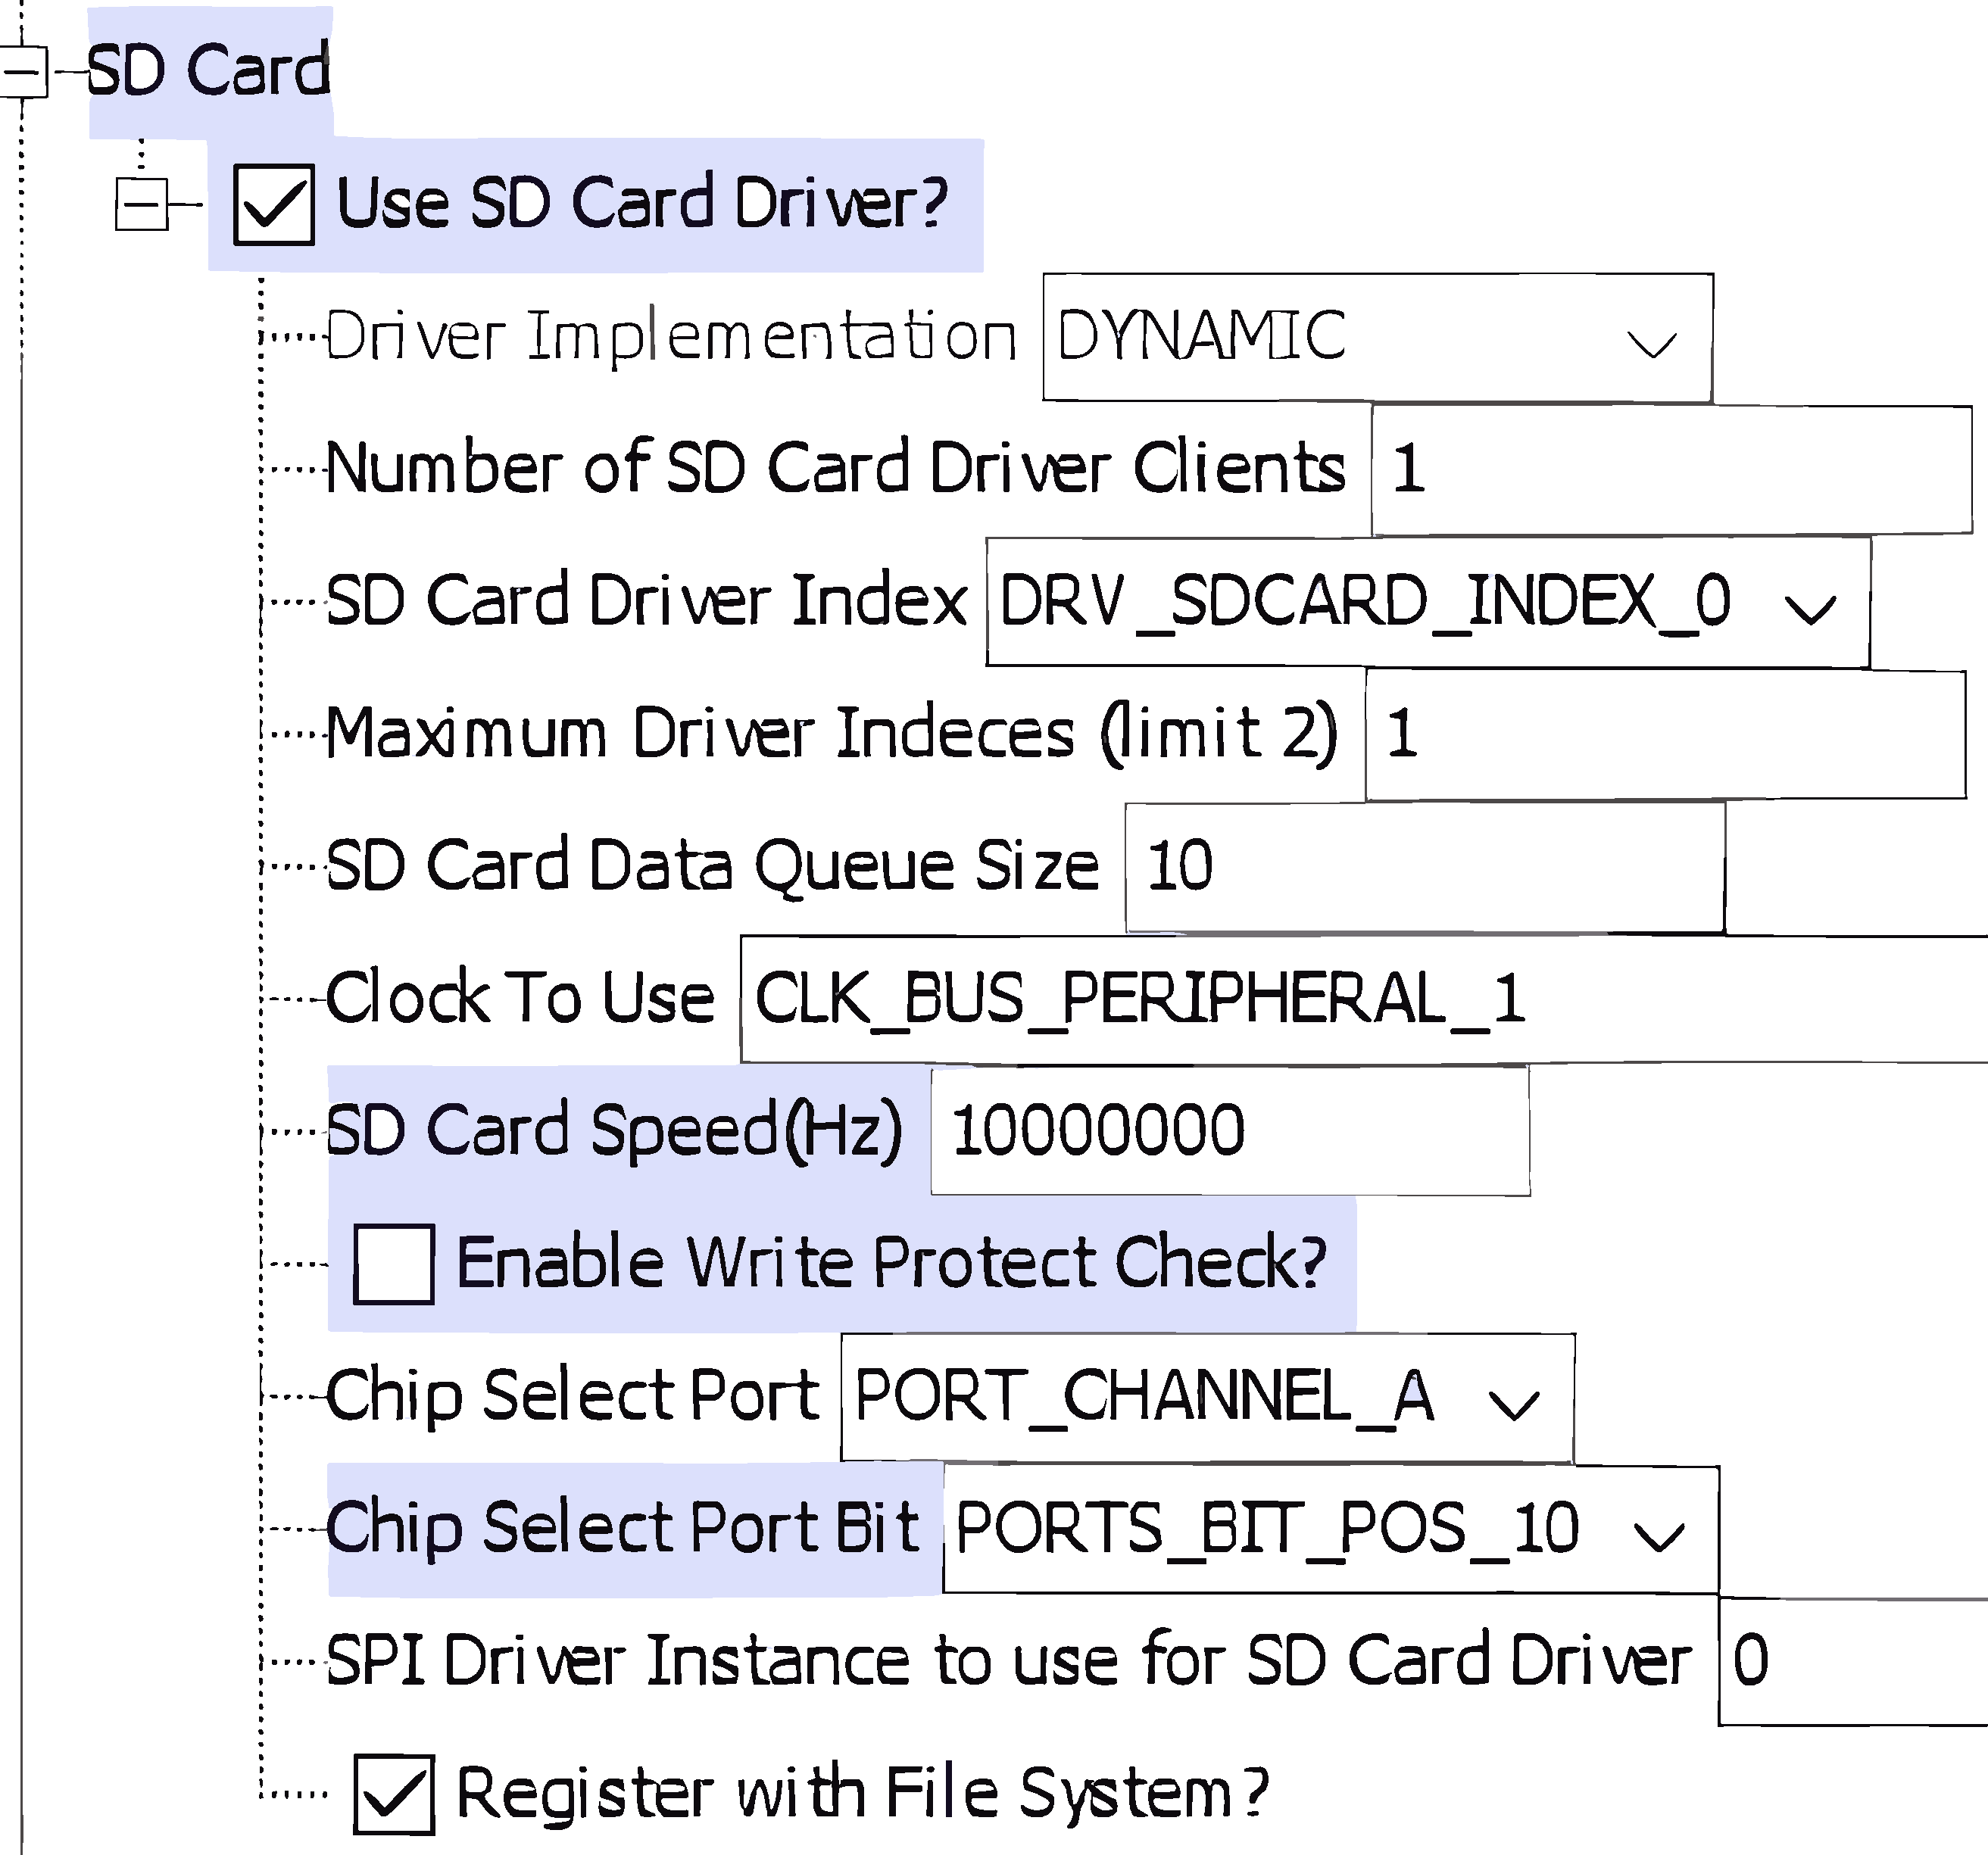
\includegraphics[width=\linewidth]{../figures/code/harmony/SD-card}
		\caption{Configuration Carte SD.}
		\label{fig:sd-card}
	\end{subfigure}
	\hfill
	\begin{subfigure}[b]{0.44\textwidth}
		\centering
		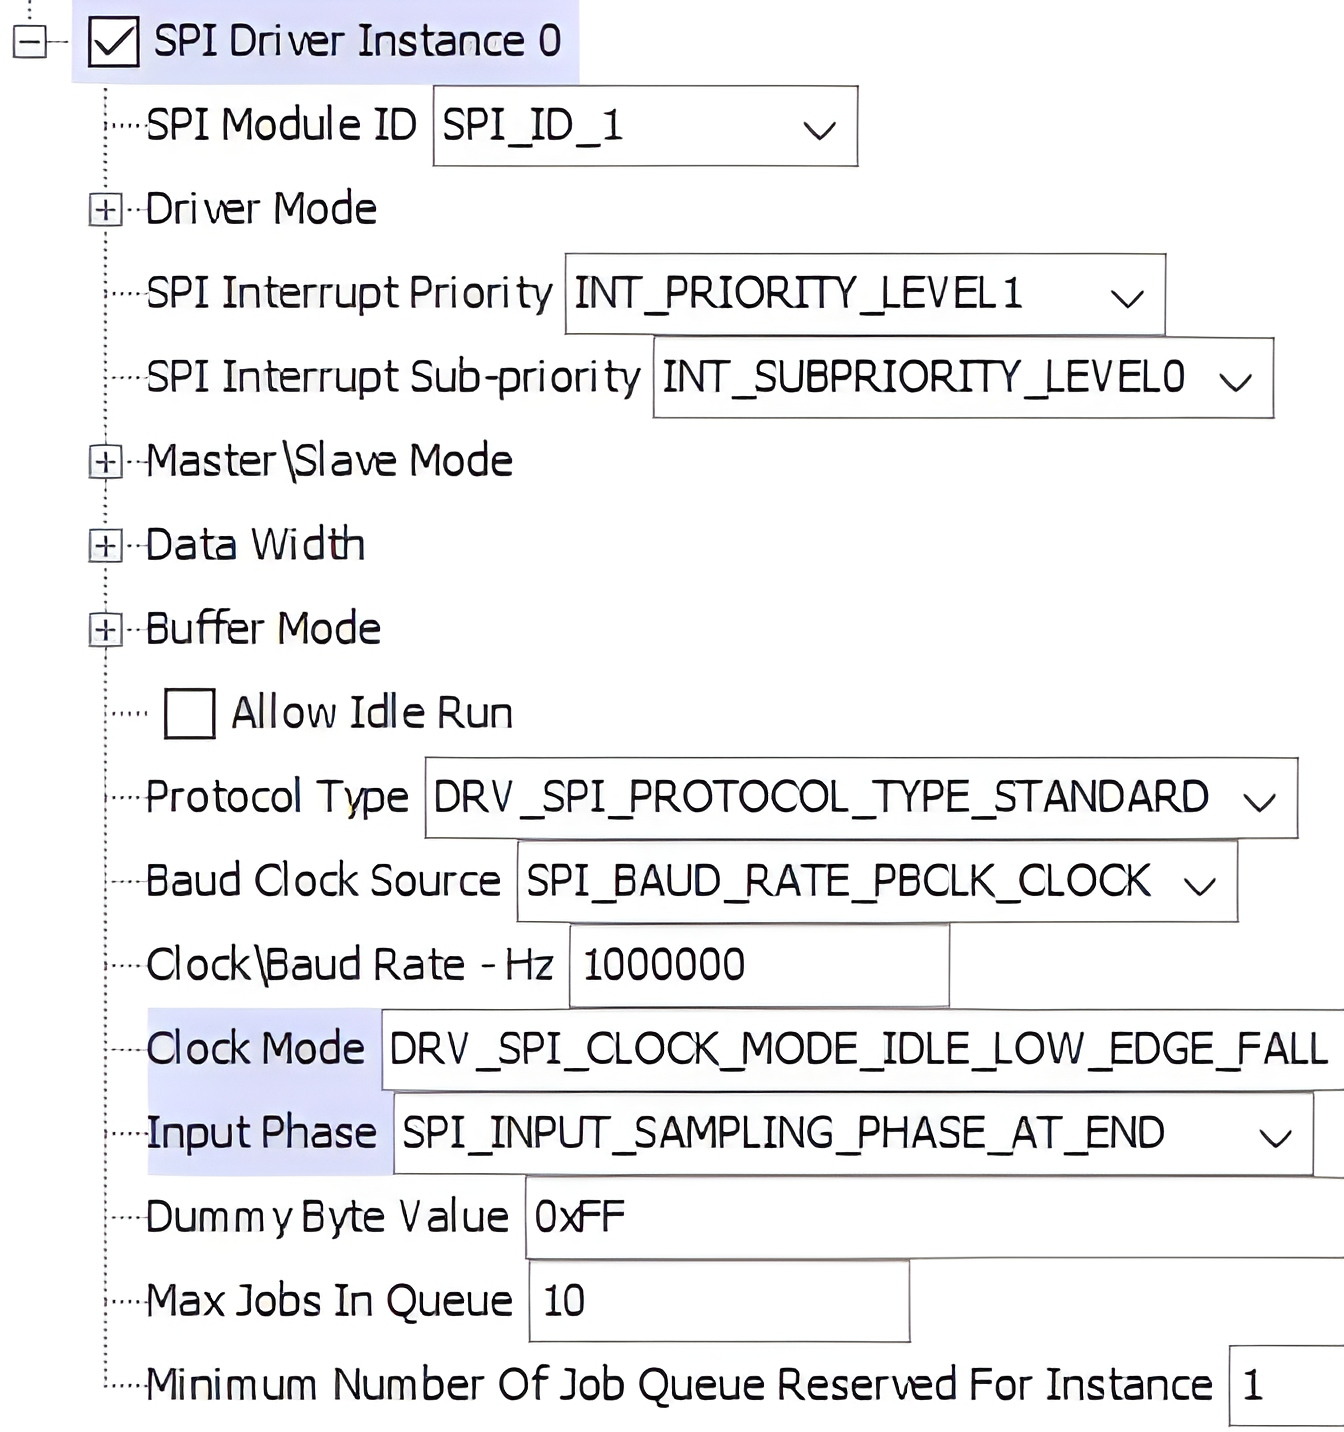
\includegraphics[width=\linewidth]{../figures/code/harmony/SD-card-spi}
		\caption{Configuration SPI.}
		\label{fig:sd-card-spi}
	\end{subfigure}
	\hfill
	\caption{Harmony, driver carte-SD.}
	\label{fig:HDriverSD}
	\source{Auteur}
\end{figure}

Sur la figure \ref{fig:sd-card}, on peut observer la configuration de la carte SD. La broche de \textit{Chip Select} est attribuée à \textbf{RA10}, qui correspond à \textbf{CS\_SD} sur le schéma présenté à la figure \ref{fig:mcu}. La connexion est établie avec une fréquence de \textbf{10MHz}.

Concernant la figure \ref{fig:sd-card-spi}, les spécificités du bus SPI y sont configurées, incluant le mode de l'horloge et la phase de l'échantillonnage. Ces configurations ont été adaptées en adéquation avec les protocoles des cartes SD\footnote{\href{https://www.renesas.com/us/en/document/apn/sd-memory-card-interface-using-spi}{SD Memory Card Interface Using SPI}.}.


\clearpage

\subsection{Application principale} 

Lors de cette section nous allons décrire le fonctionnement principale du système sous la forme d'un diagramme d'état sur la figure \ref{fig:stateapp}.

\begin{figure}[h]
	\centering
	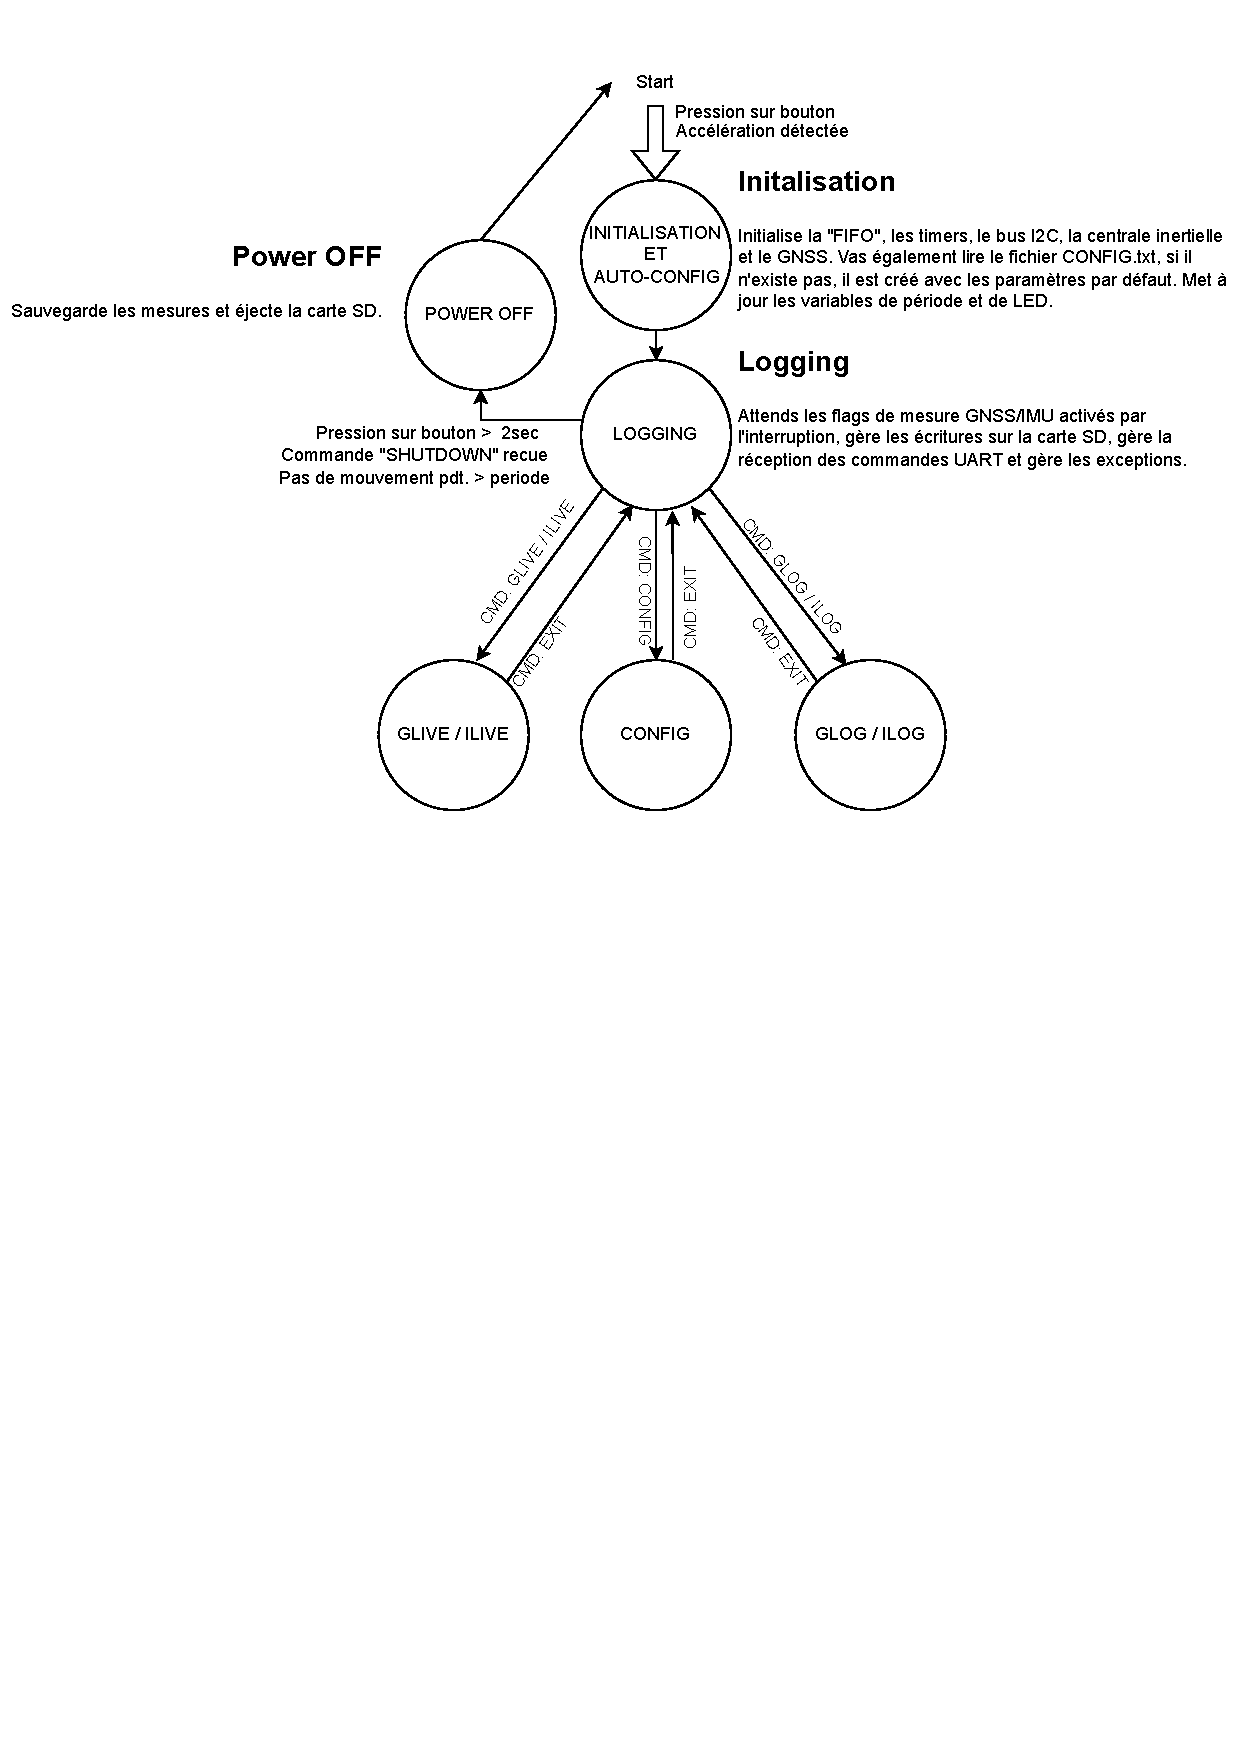
\includegraphics[width=1\linewidth]{../figures/code/diagrammes/state_app}
	\caption{Diagramme d'état principal.}
	\label{fig:stateapp}
	\source{Auteur}
\end{figure}

\subsubsection{Commandes USB-UART}
Les commandes permettent d'interagir avec le système et de manipuler les différentes données de la boîte noire.

\begin{center}
	\underline{Liste des commandes}
	\begin{table}[h]
		\centering
		\resizebox{\textwidth}{!}{
			\begin{tabular}{llll}
			GLIVE & -LVG & : & Permet d'afficher les données du \gls{gnss} en live sur le terminal sans les enregistrer. \\
			ILIVE & -LVI & : & Lance l'envoi des données live de l'\gls{imu} sans les enregistrer. \\
			GLOG & -GL & : & Envoie les données de localisation de la carte-SD au terminal. \\
			ILOG & -IL & : & Envoie les données inertielle de la carte-SD au terminal.\\
			GCLR & -GC & : & Supprime les logs du \gls{gnss}.\\
			ICLR & -IC & : & Supprime les logs de l'\gls{imu}.\\
			EXIT & X & : & Quitte le mode en cours.\\
			SHUTDOWN & -OFF & : & Sauvegarde et éteint le système. \\
			CONFIG & -CFG & : & Démarre le mode de configuration du système. \\
			\faChevronRight & INTG:XXXX & : & Dans mode config. permet de régler la période de mesure du \gls{gnss}.\\
			\faChevronRight & INTI:XXXX & : & Dans mode config. permet de régler la période de mesure de l'\gls{imu}. \\
			\faChevronRight & LEDV:X & : & Dans mode config. permet d'activer ou non la LED de vie. \\
			\faChevronRight & TOFF:XX & : & Dans mode config. permet de fixer le temps d'inactivité (éteint le système).
		\end{tabular}
		}
		\caption{Commandes disponibles}
		\label{tab:cmdDisp}
	\end{table}
\end{center}

Les commande de la table \ref{tab:cmdDisp} peuvent également être envoyés en caractères minuscules.

\clearpage

Sur la figure \ref{fig:sequence-app}, la séquence de la boucle principale de l'application est représentée. Celle-ci interagit avec les différents périphériques en utilisant diverses bibliothèques C.

\begin{figure}[!h]
	\centering
\	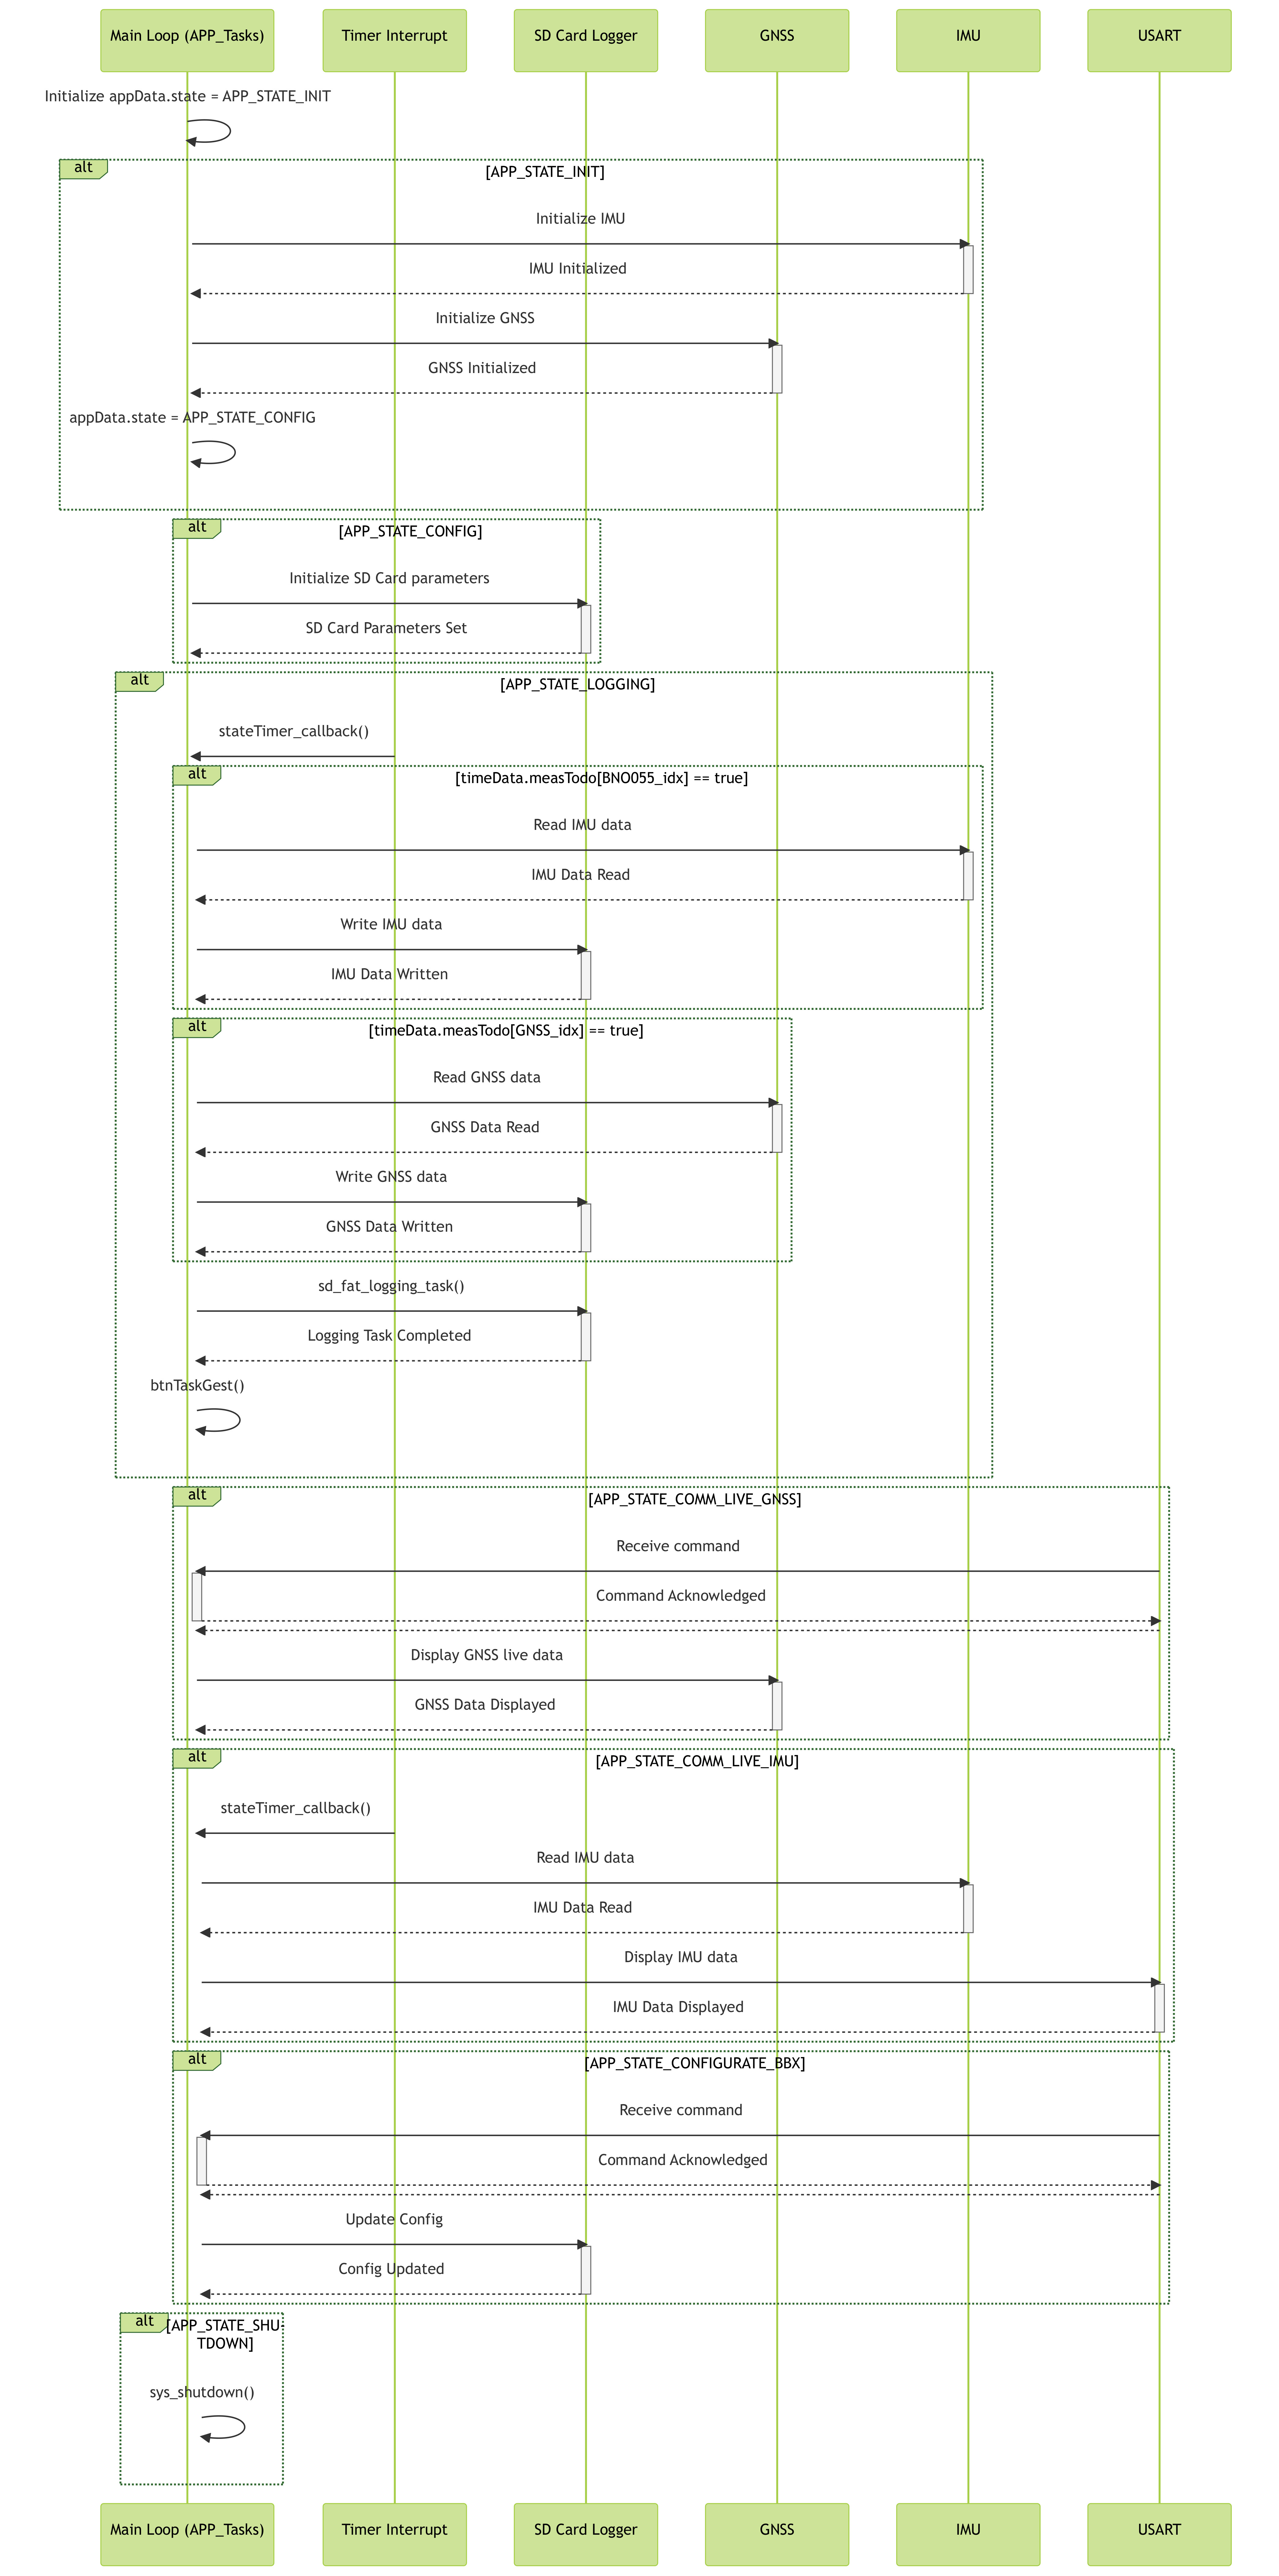
\includegraphics[width=.96\linewidth]{../figures/code/diagrammes/sequence-app}
	\caption{Diagramme de séquence principal.}
	\label{fig:sequence-app}
	\source{Auteur}
\end{figure}

\clearpage
\subsubsection{État de logging du système}
L'état de logging est représenté par un flowchart sur la figure \ref{fig:pdfresizer}.

\begin{figure}[!h]
	\centering
	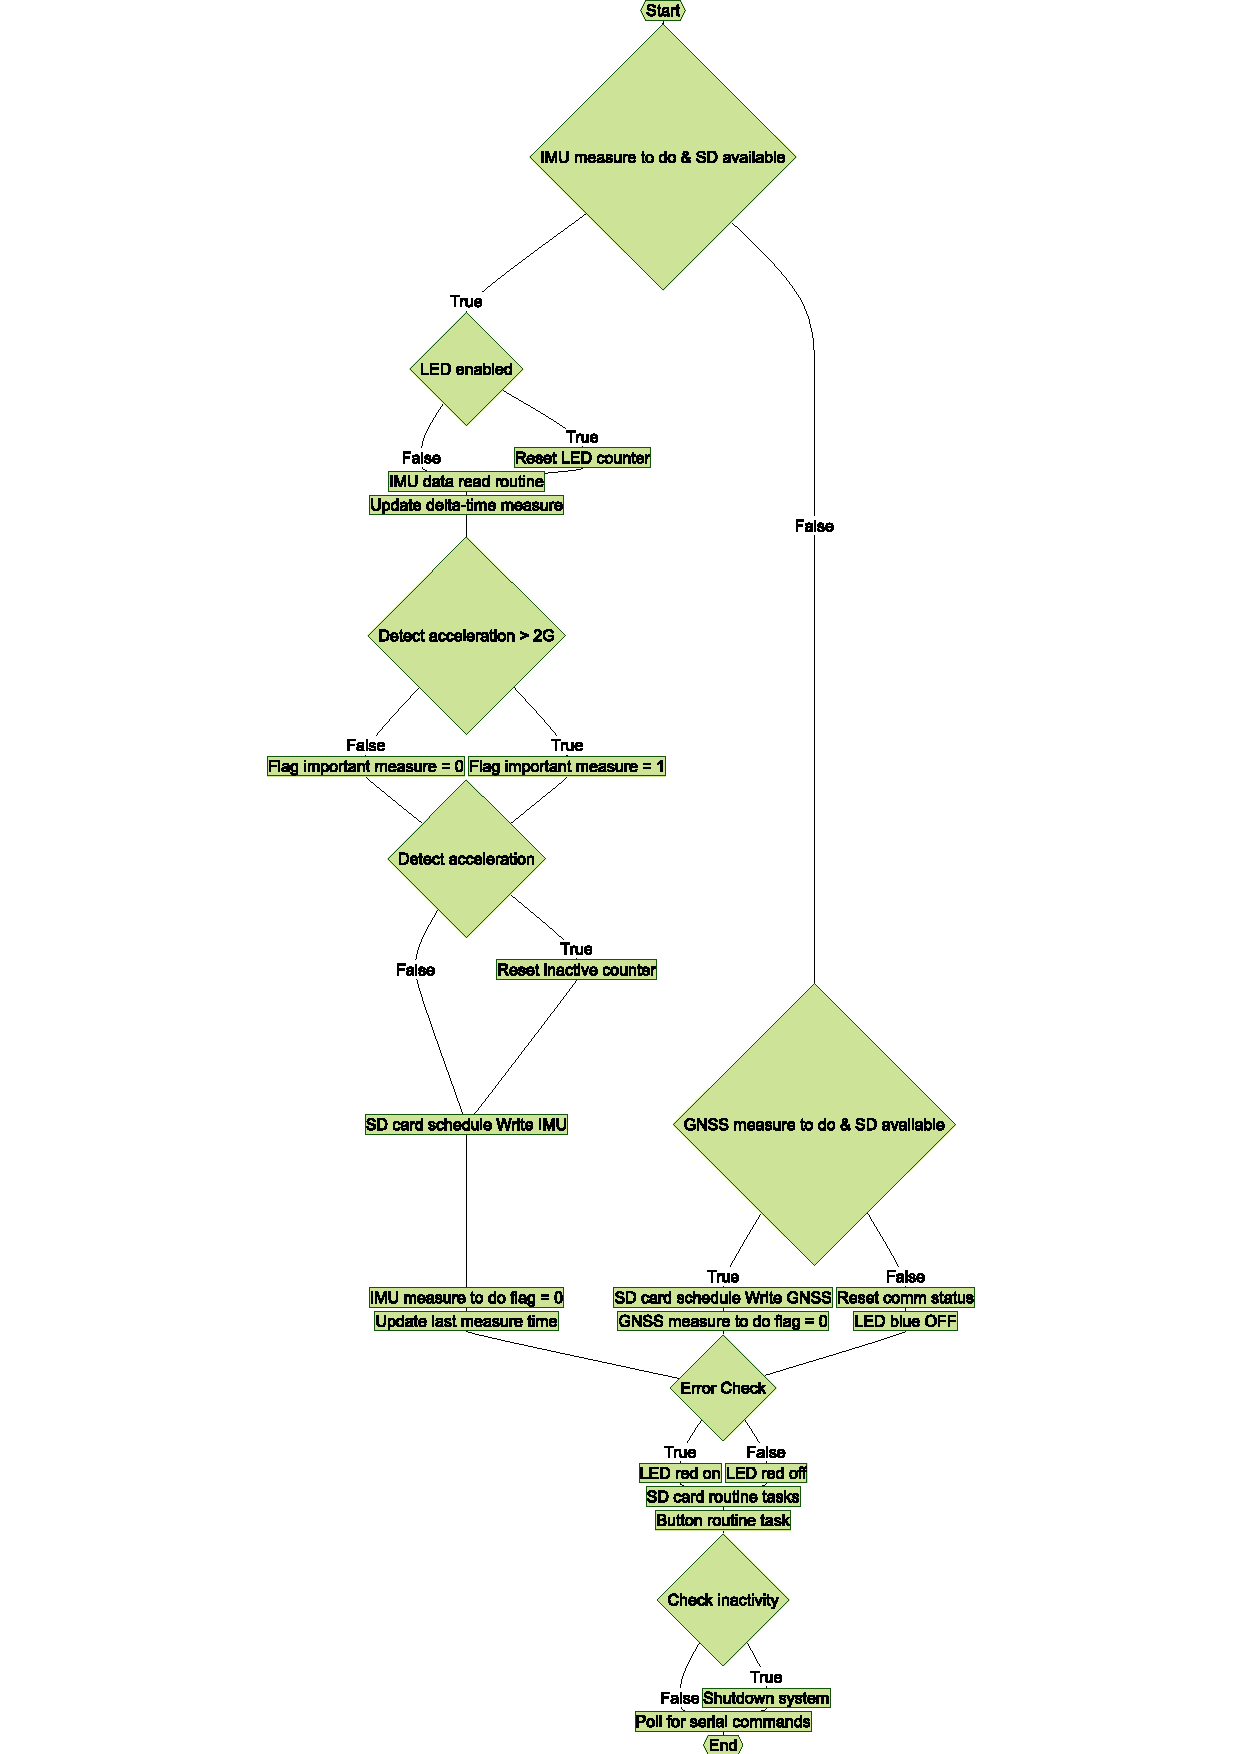
\includegraphics[width=.95\textwidth]{../figures/code/diagrammes/logging-flowchart}
	\caption{Flowchart de l'état de logging.}
	\label{fig:pdfresizer}
	\source{Auteur}
\end{figure}

\clearpage

\subsection{Carte SD}
Le code de gestion de fichier de la carte SD est divisé en deux machines d'états. La première est dédiée à l'initialisation, à la lecture et à la modification du fichier de configuration. La seconde s'occupe du logging et de l'enregistrement des mesures dans des fichiers distincts. Ces machines d'états sont non-bloquantes et doivent être appelées périodiquement pour permettre une routine de gestion de la carte SD.

\subsubsection{Carte SD : initialisation et configuration}

La machine d'état initiale est appelée lorsqu'elle se trouve dans l'état \textbf{APP\_STATE\_CONFIG}, comme illustré sur la figure \ref{fig:sequence-app}. Elle continuera d'être appelée jusqu'à ce qu'elle atteigne l'état \textbf{\textit{IDLE}}. Notons également que cette machine d'état est sollicitée en mode configuration (\textbf{\textit{init = false}}) durant l'état \textbf{APP\_STATE\_CONFIGURATE\_BBX}, visible sur la même figure \ref{fig:sequence-app}. Ce processus est représenté sous forme de diagramme d'état à la figure \ref{fig:sd-card-init}



\begin{figure}[h]
	\centering
	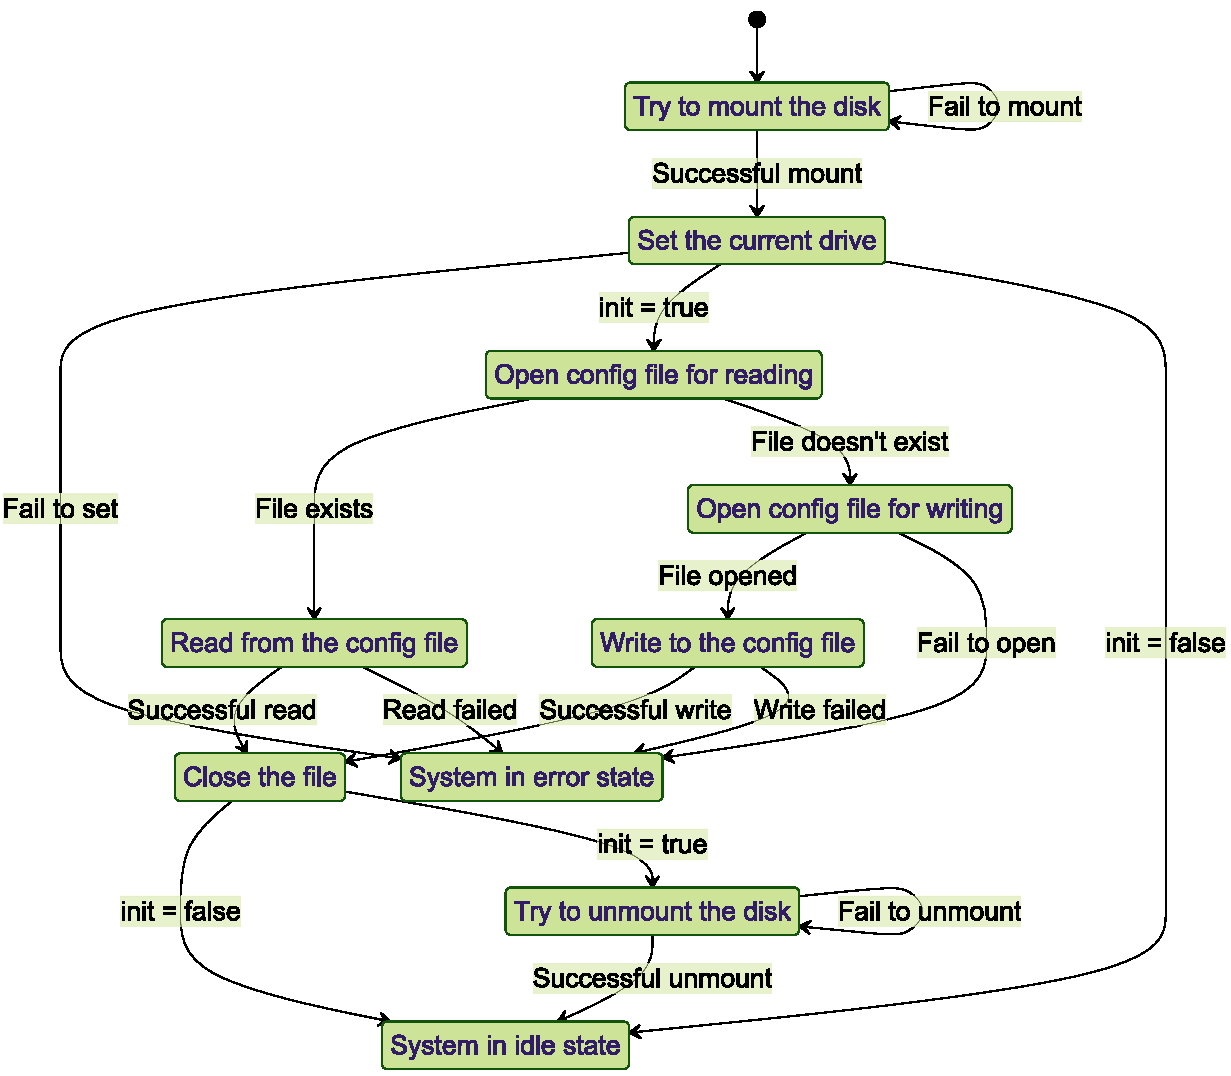
\includegraphics[width=1\linewidth]{../figures/code/diagrammes/sd-card-Init}
	\caption{Application carte SD initialisation/config.}
	\label{fig:sd-card-init}
	\source{Auteur}
\end{figure}

\clearpage

\subsubsection{Carte SD : écriture des données}
Cette machine d'état est systématiquement appelée lorsque le système se trouve dans l'état \textbf{APP\_STATE\_LOGGING}, comme illustré sur la figure \ref{fig:sequence-app}. Ceci est réalisé via la fonction \verb*|sd_fat_logging_task()|. Pour programmer des écritures et interagir avec cette machine d'état, deux fonctions d'interface sont utilisées : \verb*|sd_IMU_scheduleWrite()| qui permet de planifier l'écriture de données de l'\gls{imu}, et \verb*|sd_GNSS_scheduleWrite()| pour l'écriture des données du \gls{gnss}.

\begin{figure}[h]
	\centering
	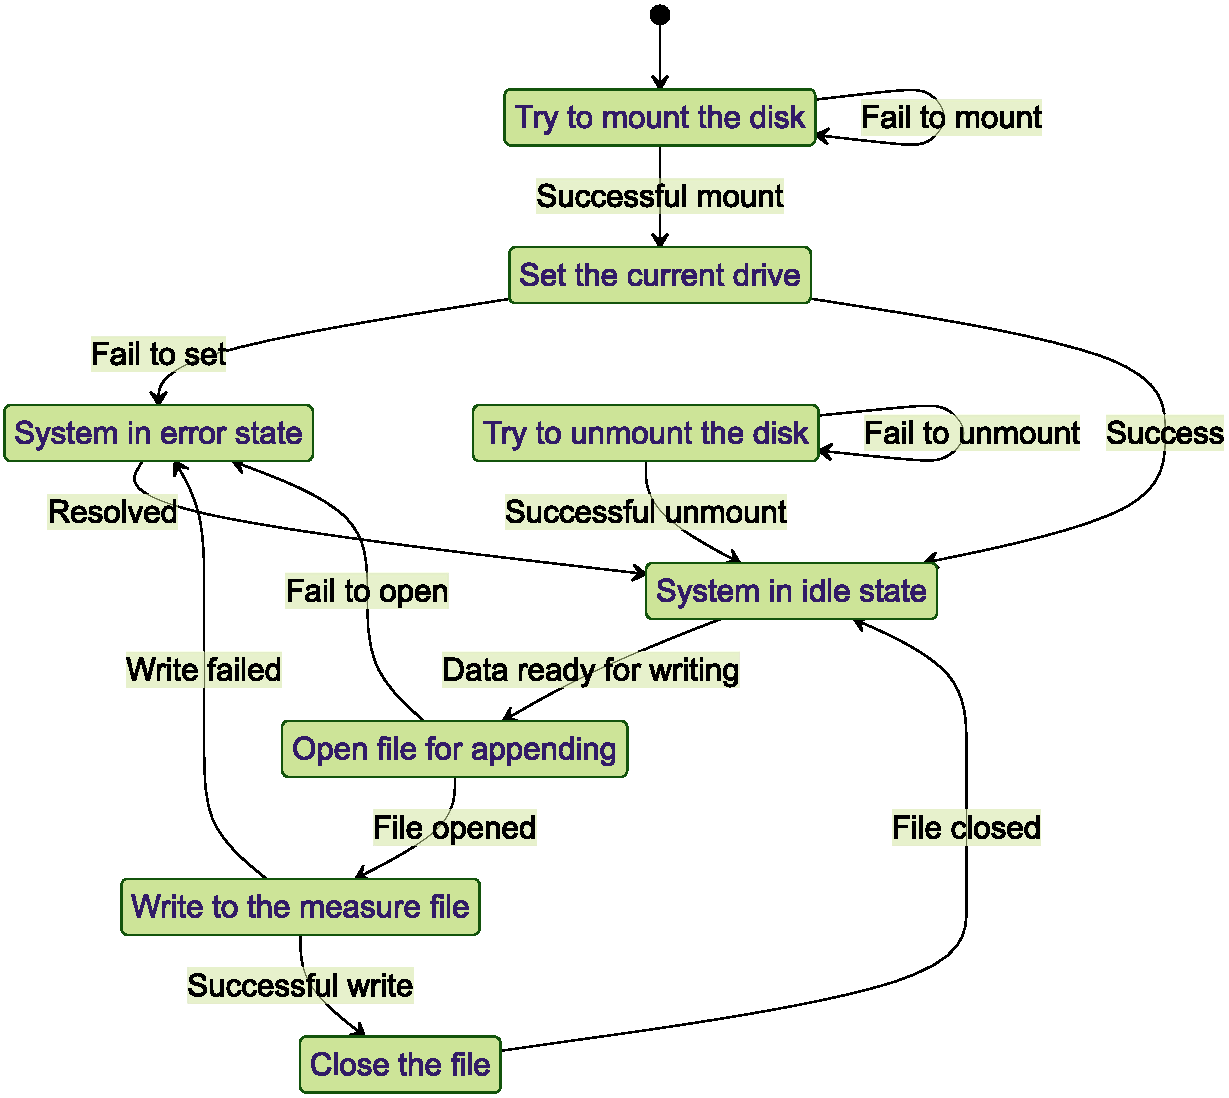
\includegraphics[width=.85\linewidth]{../figures/code/diagrammes/sd-card-logging}
	\caption{Machine d'état logging.}
	\label{fig:sd-card-logging}
	\source{Auteur}
\end{figure}

\begin{figure}[h]
	\centering
	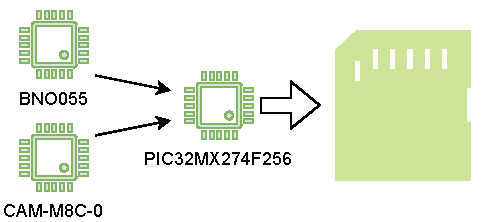
\includegraphics[width=0.46\linewidth]{../figures/code/Illustration-SD-per}
	\caption{Illustration des interactions.}
	\label{fig:illustration-sd-per}
	\source{Auteur}
\end{figure}

\clearpage

\subsection{Centrale inertielle}
Lors de cette section, nous allons décrire les différents aspects de la mise en place de la centrale inertielle \fbox{\href{https://www.bosch-sensortec.com/products/smart-sensors/bno055/}{BNO055}}.

\paragraph*{Interfaçage de l'\gls{imu}}
Bosch propose une librairie\footnote{\href{https://github.com/BoschSensortec/BNO055_driver}{https://github.com/BoschSensortec/BNO055\_driver}} d'APIs pour communiquer avec la centrale inertielle. Cette librairie est accompagnée d'un fichier \textit{support} qui sert à lier les fonctions de protocoles aux fonctions bas niveau du bus de communication I2C.


\subsubsection{Initialisation}

\begin{center}
	\underline{Procédure d'initialisation}
	\begin{table}[h]
		\centering
		\begin{tabular}{ll}
			$\star$ \oldstylenums{1} & Réinitialisation hardware par la pin RESET pendant 100ms. \\
			$\star$ \oldstylenums{2} & Désactivation de l'interruption\footnotemark de l'\gls{imu}. \\
			$\star$ \oldstylenums{3} & Attribution des fonctions bas niveau dans les pointeurs de la librairie. \\
			$\star$ \oldstylenums{4} & Obtention des informations du BNO055 (IDs, Version...). \\
			$\star$ \oldstylenums{5} & Attribution du mode d'alimentation "Normal". \\
			$\star$ \oldstylenums{6} & Choix du mode d'opération "AMG" (pour lecture simple Accel. magnitude et gyro.). \\
			$\star$ \oldstylenums{7} & Lecture initiale à vide, d'initialisation (Accel. magnitude gyroscope.). \\
			$\star$ \oldstylenums{6} & Choix du mode d'opération "NDOF" (pour lecture des données de fusions complexes.). \\
			$\star$ \oldstylenums{7} & Lecture initiale à vide, d'initialisation (Euler, Quaternion, gravité et accel. linéaire). \\
			$\star$ \oldstylenums{8} & Programmation de l'interruption du BNO055 pour la détection d'une certaine accélération.
		\end{tabular}
	\end{table}
\end{center}
\footnotetext{Reset toutes les sources d'interruptions de l'\gls{imu} dans le registre 0x3F bit 6. }
\vspace*{-15mm}

\subsubsection{Lecture des données}

La phase cruciale concernait l'initialisation du BNO055. La lecture des diverses valeurs est assurée par une fonction spécifiquement créée, nommée \verb*|bno055_read_routine()|. Cette fonction récupère les données suivantes : Quaternion WXYZ, magnitude XYZ, gyroscope XYZ, angles d'Euler HPR, accélération linéaire XYZ, et gravité XYZ. Ces données son stockées dans une structure locale au fichier \textit{app.c} et possède la structure suivante :

\begin{minted}{c}
typedef struct {
	s32 comres;
	bool flagMeasReady;
	uint8_t flagImportantMeas;
	struct bno055_gravity_double_t gravity;
	struct bno055_linear_accel_double_t linear_accel;
	struct bno055_euler_double_t euler;
	struct bno055_gyro_double_t gyro;
	struct bno055_mag_double_t mag;
	struct bno055_quaternion_t quaternion;
	unsigned long time;
	unsigned long l_time;
	uint16_t d_time;
}s_bno055_data;
\end{minted}

\subsubsection{Système de détection de mouvements}

La centrale inertielle \textit{BNO055} permet de configurer une interruption pour un certain événement et une certaine durée. Dans cette section, nous décrirons la configuration de cette interruption pour l'enclenchement du système ainsi que la possibilité d'activer/désactiver cette option.

\begin{code}
\caption{Configuration de l'interruption}
\label{code:configInt}
\begin{minted}[breaklines]{c}
/* BNO055 motion interrupt mode */
1) bno055_set_accel_any_motion_no_motion_axis_enable (BNO055_ACCEL_ANY_MOTION_NO_MOTION_X_AXIS, 1);
2) bno055_set_accel_any_motion_no_motion_axis_enable (BNO055_ACCEL_ANY_MOTION_NO_MOTION_Y_AXIS, 1);
3) bno055_set_accel_any_motion_no_motion_axis_enable (BNO055_ACCEL_ANY_MOTION_NO_MOTION_Z_AXIS, 1);

4) bno055_set_accel_any_motion_thres(10);
5) bno055_set_accel_any_motion_durn(20);
6) bno055_set_intr_accel_any_motion(1);
7) bno055_set_intr_mask_accel_any_motion(1);	
\end{minted}
\end{code}

Les valeurs de configuration peuvent êtres définies en tant que constantes pour êtres plus facilement configurable lors de mise-à-jour firmware.

\begin{center}
	\underline{Description des lignes du code \ref{code:configInt}}
	\begin{table}[h]
		\centering
		\begin{tabular}{ll}
			$\star$ \oldstylenums{1} & Activation de l'axe X pour le mode \textit{anymotion}. \\
			$\star$ \oldstylenums{2} & Activation de l'axe Y pour le mode \textit{anymotion}. \\
			$\star$ \oldstylenums{3} & Activation de l'axe Z pour le mode \textit{anymotion}. \\
			$\star$ \oldstylenums{4} & Attribution de la valeur de déclenchement à $78.3 m\textbf{g} = 0.768 m/s^2$. \\
			$\star$ \oldstylenums{5} & Configuration de la durée à $20ms$. \\
			$\star$ \oldstylenums{6} & Active l'interruption, accélération. \\
			$\star$ \oldstylenums{7} & Masque l'interruption. \\
		\end{tabular}
	\end{table}
\end{center} \vspace*{-10mm}

\paragraph{Gestion de l'interruption} L'interruption est réinitialisée au démarrage du système ainsi que lors de sa mise en veille.
\vspace*{-4mm}
\paragraph{Mode low power} lorsque le système se met en veille, la BNO055 est configurée pour fonctionner uniquement avec son accéléromètre et son mode de puissance passe en \textit{low power}.

\begin{code}
\caption{Configuration de l'interruption}
\label{code:lowPowerBNO}
\begin{minted}[breaklines]{c}
/* Set acceleration only operation, power saving */
bno055_set_operation_mode(BNO055_OPERATION_MODE_ACCONLY);
/* set the power mode to LOW POWER */
bno055_set_power_mode(BNO055_POWER_MODE_LOWPOWER);
/* Reset interrupt pin */
bno055_set_intr_rst(1);	
\end{minted}
\end{code}

\clearpage

\paragraph{Configuration enclenchement automatique}

Le système propose deux modes d'opération : le premier permet un enclenchement automatique lors de la détection d'un mouvement, tandis que le second active le système suite à une impulsion sur le bouton. Il est à noter que pour activer le mode automatique, une première impulsion sur le bouton est nécessaire et le système doit avoir transité au moins une fois par l'état "shutdown" du code. Dans les deux modes, le système peut entrer en veille si aucun mouvement n'est détecté sur une durée configurée.

Lorsque le système est en mode d'enclenchement automatique, le circuit reste partiellement actif, ce qui engendre une consommation d'énergie détaillée ultérieurement dans la section "Validation du design". Même si la batterie est en mesure de supporter cette consommation, il reste possible de désactiver ce mode pour activer le système uniquement par le biais du bouton.

\paragraph*{Configuration} La centrale inertielle peut être alimentée soit de manière indépendante, soit avec le reste du système, influençant ainsi les modes décrits précédemment. Pour configurer ces modes, deux options sont disponibles : \vspace*{+2mm}


\begin{tabular}{lll}
	\textbf{W6} connecté & \gls{imu} alimentation autonome. & Mode accélération auto-enclenchement. \\
	\textbf{W7} connecté & Alimentation dépendant du système. & Mode enclenchement bouton uniquement. \\
	\textbf{W6} \& \textbf{W7} & \color{red}{Connexion à éviter !} & \\
\end{tabular}

\begin{figure}[h]
	\centering
	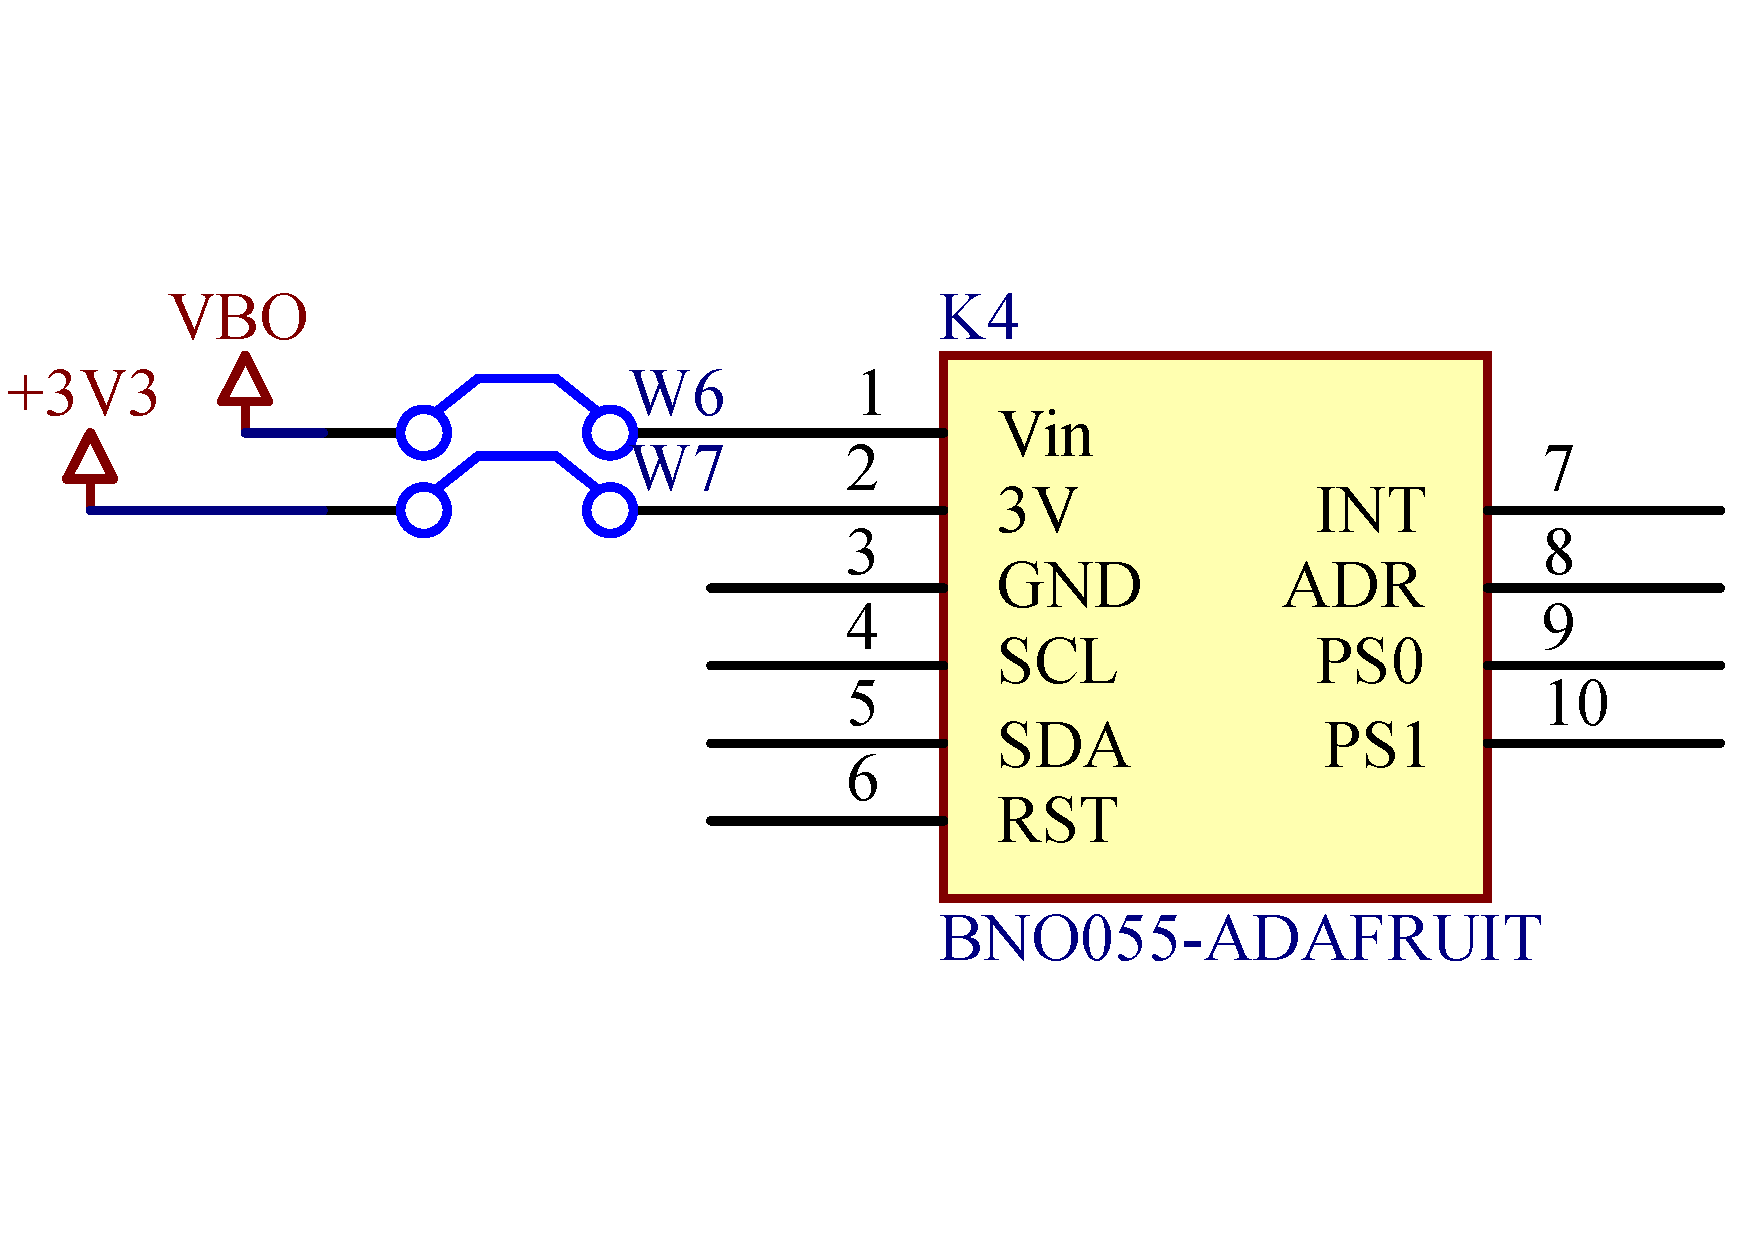
\includegraphics[width=0.7\linewidth]{../figures/code/jumper-config-mode-IMU}
	\caption{Connexions des jumber du BNO055.}
	\label{fig:jumper-config-mode-imu}
\end{figure}

\begin{figure}[h]
	\centering
	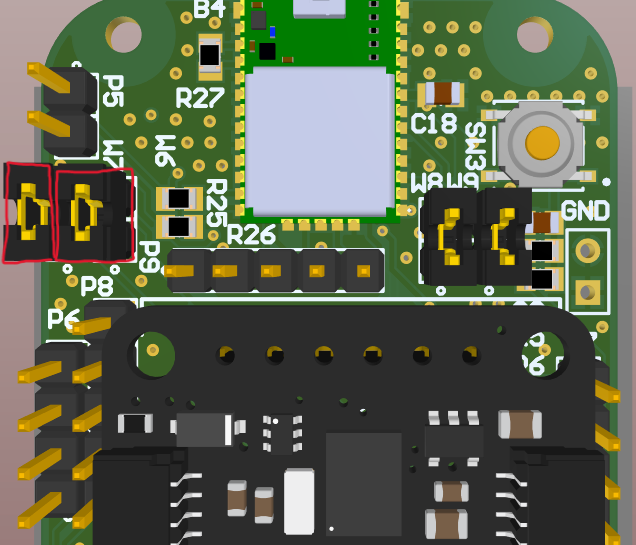
\includegraphics[width=0.5\linewidth]{../figures/code/config-mode-IMU}
	\caption{Emplacement des jumpers sur le \gls{pcb}.}
	\label{fig:config-mode-imu}
\end{figure}

Sur la figure \ref{fig:config-mode-imu}, les jumpers sont entourés en \textbf{rouge}. Le jumper \textbf{W6} se situe à droite tandis que \textbf{W7} se situe à gauche.

\clearpage	

\subsection{Format des données}

Lors de cette section, sera décrite les formats des données enregistrer dans la carte SD.

\subsubsection{Données de l'IMU} 

\subsubsection{Données du GNSS} 

\subsection{Hiérarchie des fichiers du système}




